\documentclass[a5paper,openany]{book}


\usepackage[utf8]{inputenc}
\usepackage[T1]{fontenc}
\usepackage[english]{babel}

% set font to Linux Libertine (non-proprietary font):
% this requires downloading the font, e.g., from
%    https://sourceforge.net/projects/linuxlibertine/
% and installing it manually
% then, compile using xelatex paperwriting.tex
% \usepackage{fontspec}
% \setmainfont{Linux Libertine O}
% alternative for pdflatex (does not work with certain font variants)
\usepackage{libertine}

%\usepackage[pass]{geometry}  % to make a5paper work
\usepackage[a5paper,bottom=3cm]{geometry}

\usepackage{setspace}
\setstretch{1.2}  % default value: 1.44

% \usepackage{tocloft}

\usepackage{mathtools,amsfonts}  % for math (loads amsmath, amsfonts(?), amssymb)

\usepackage{pifont}  % for checkmark, cross
\usepackage{siunitx}  % for SI units guideline

\usepackage{xcolor}  % customized colors
\usepackage[most]{tcolorbox}  % for guidelines and examples
\tcbuselibrary{skins}  % enhanced formatting for tcolorbox
\tcbuselibrary{raster}  % for good/bad examples

\usetikzlibrary{arrows}
\tikzset{
	myarrow/.style={<-, shorten <=0.05cm, >=stealth', semithick}
}

\usepackage{enumitem}

\usepackage{booktabs}  % tables
\usepackage{multirow}  % tables
\usepackage{longtable}  % for table of references for guidelines

\usepackage{soul}  % for highlighting multiline text

\usepackage{fancyhdr}  % for formatting headers
\pagestyle{fancy}  % enable custom header functionality
\renewcommand{\headrulewidth}{0pt}  % no horizontal line below header

\fancyhead[L]{\thepage}  % left header: page number
\fancyhead[C]{}
\fancyhead[R]{\nouppercase{\leftmark}}  % right header: chapter number and name
\fancyfoot[L]{}
\fancyfoot[C]{}
\fancyfoot[R]{}

% glossary / list of terms
\usepackage[nopostdot]{glossaries}
\newglossaryentry{emphasis}{name = {emphasis}, description={}}
%% \setglossarystyle{list}
%% \makeglossaries


\usepackage{csquotes}  % required by compilation?
\usepackage[backend=biber,
    url=false,
    doi=true,
    isbn=true,
    style=ext-numeric-comp,
    defernumbers=true,
    %giveninits,
    sorting=none,
    maxnames=100]{biblatex}
\addbibresource{tex/references.bib}

\DeclareFieldFormat{titlecase:title}{\MakeSentenceCase*{#1}}
\DeclareFieldFormat{titlecase:booktitle}{#1}
\DeclareFieldFormat{titlecase:journaltitle}{#1}
\DeclareFieldFormat{doi}{doi: \text{#1}}

% colors for boxes
\definecolor{color_guideline}{RGB}{0, 92, 171}
\definecolor{color_guideline_background}{rgb}{0.588, 0.784, 0.902}
\definecolor{color_example_frame}{rgb}{0.65,0.65,0.65}
\definecolor{color_highlight}{RGB}{255, 195, 37}
% \definecolor{color_example_good}{rgb}{0.4706,0.7725,0.4980}
% \definecolor{color_example_bad}{rgb}{0.9059,0.7373,0.7373}

\definecolor{color_example_good}{HTML}{228B22}
\definecolor{color_example_bad}{HTML}{B22222}


% guidelines
\newcounter{guidelinecounter}
\newcommand{\guideline}[3][defaultguidelinelabel]{%
\refstepcounter{guidelinecounter}
\label{#1}
\begin{tcolorbox}[
    title=Guideline \theguidelinecounter.,
    colback=color_guideline_background, colframe=color_guideline,
    sharp corners=northwest,bottomrule=0mm,rightrule=0mm,leftrule=0mm,
    left=2mm,right=2mm]
    #2
\end{tcolorbox}%
\addcontentsline{toc}{section}{Guideline \theguidelinecounter. #2}
}

% text example for comparison good/bad (two columns)
\newcommand{\goodbadexample}[3][]{%
\ifx\relax#1\relax
\begin{tcbraster}[raster row skip=3pt,raster columns=1]
\begin{tcolorbox}[enhanced,breakable,frame hidden,interior hidden,colback=white,
    borderline west={0.75mm}{0.25mm}{color_example_bad},
    top=0mm,bottom=0mm,right=0mm,left=2.5mm]
    #2
\end{tcolorbox}
\begin{tcolorbox}[enhanced,frame hidden,interior hidden,colback=white,
    borderline west={0.75mm}{0.25mm}{color_guideline},
    top=0mm,bottom=0mm,right=0mm,left=2.5mm]
    #3
\end{tcolorbox}%
\end{tcbraster}%
\else
{\hfill \scriptsize{#1}}
\begin{tcbraster}[raster before skip=0pt,raster row skip=3pt,raster columns=1]
\begin{tcolorbox}[enhanced,breakable,frame hidden,interior hidden,colback=white,
    borderline west={0.75mm}{0.25mm}{color_example_bad},
    top=0mm,bottom=0mm,right=0mm,left=2.5mm]
    #2
\end{tcolorbox}
\begin{tcolorbox}[enhanced,frame hidden,interior hidden,colback=white,
    borderline west={0.75mm}{0.25mm}{color_guideline},
    top=0mm,bottom=0mm,right=0mm,left=2.5mm]
    #3
\end{tcolorbox}%
\end{tcbraster}%
\fi%
}

% text example (single column)
\newcommand{\badexample}[2][]{%
\ifx\relax#1\relax
\begin{tcolorbox}[enhanced,breakable,frame hidden,interior hidden,colback=white,
    borderline west={0.75mm}{0.25mm}{color_example_bad},
    top=0mm,bottom=0mm,right=0mm,left=2.5mm]
    #2
\end{tcolorbox}%
\else
{\hfill \scriptsize{#1}}
\begin{tcolorbox}[before skip=0pt,
    enhanced,breakable,frame hidden,interior hidden,colback=white,
    borderline west={0.75mm}{0.25mm}{color_example_bad},
    top=0mm,bottom=0mm,right=0mm,left=2.5mm]
    #2
\end{tcolorbox}%
\fi%
}
\newcommand{\goodexample}[2][]{%
\ifx\relax#1\relax
\begin{tcolorbox}[enhanced,breakable,frame hidden,interior hidden,colback=white,
    borderline west={0.75mm}{0.25mm}{color_guideline},
    top=0mm,bottom=0mm,right=0mm,left=2.5mm]
    #2
\end{tcolorbox}%
\else
{\hfill \scriptsize{#1}}
\begin{tcolorbox}[before skip=0pt,
    enhanced,breakable,frame hidden,interior hidden,colback=white,
    borderline west={0.75mm}{0.25mm}{color_guideline},
    top=0mm,bottom=0mm,right=0mm,left=2.5mm]
    #2
\end{tcolorbox}%
\fi%
}

% highlight background of crucial parts
\sethlcolor{color_highlight}
\newcommand{\highlightpart}[1]{\hl{#1}}
\newcommand{\highlightempty}{\hl{ }}
\newcommand{\highlightpartmath}[1]{\text{\highlightpart{$#1$}}}  % soul can run into problems in math env

% row in table of references for guidelines
\newcommand{\guidelineref}[2]{\ref{#1} & \fullcite{#2} \\}


%%%% titlepage
\title{\huge Guidelines for Scientific Paper Writing in Computer Science}
\author{\Large Mark Wetzlinger}
\date{}
%%%%


\begin{document}

%%%% TITLE, ACKS, PREFACE, TOC %%%%
\frontmatter

\maketitle

\chapter*{Acknowledgments}

First and foremost, I want to express my gratitude to my advisor Matthias and my mentor Niklas, who taught me most of what I know.
Many thanks also to my wonderful group of colleagues, and in particular Hanna, for mutual proofreading over many years as well as countless discussions on the craft of paper writing.
% Special thanks to Tobias and Max for proofreading this manuscript.

\bigskip

\noindent Munich, November 2024 \hfill Mark Wetzlinger%
\chapter*{Preface}

Publishing papers is essential to pursuing a doctoral degree.
While conducting research is an art, where creativity and intuition lead to uncovering new insights, paper writing is a craft, demanding a methodical approach to presenting those insights clearly.

I was very fortunate to have had both a PhD supervisor and a mentor that invested time and efforts in teaching me this craft.
Besides writing papers myself, I have also proofread numerous drafts of my junior colleagues, and I have reviewed many submissions to conferences and journals.
I consider the feedback loop of writing and reviewing to be the best teacher:
Reading and reviewing papers provides examples of both good and bad, whereas the actual learning comes from being forced to make decisions in one's own work, and having gone through this process may in turn change one's perspective on how others made their decisions.

So after more than five years, I humbly claim to have understood a thing or two about the craft of paper writing.
Of course, it would be presumptuous to claim there were one way of structuring content, outlining concepts, or explaining details.
Still, these tasks often raise similar questions, soliciting similar advice.
I have thus decided to comprise my knowledge and observations in this booklet, hoping that others may find it helpful.
The word \emph{guidelines} in the title is carefully chosen, as they may guide, not impose.
Some parts may be more contentious than others, but I believe any such discussion is ultimately in the reader's best interest as an author.

A few brief words on the content:
Early chapters focus more on high-level concepts, such as structure and how to manage different levels of depth, while later chapters list specific guidelines for specific questions.
% todo: be more specific once the structure is decided (difference between part I and part II)
% todo: include restriction to non-survey papers, no book chapter, no other summaries; rather: presentation of a novel idea in a conference paper or journal article...
% todo: find out which types of papers exist
The structure of this booklet is deliberately minute to allow for feeding specific parts to AI tools so that some changes can be automated.
Please also note that the scope is limited to computer science, as I am convinced it is better to stick with what I know best.
I do hope, however, that much of the content is transferable to other research disciplines as well.

\bigskip

\noindent Thank you for reading, \\
\noindent Mark.


%% standard table of contents
\tableofcontents

%% brief contents and standard table of contents
% \clearpage

% \setcounter{tocdepth}{0}
% \renewcommand{\contentsname}{Brief Contents}
% \setlength{\cftbeforepartskip}{10pt}
% \setlength{\cftbeforechapskip}{2pt}
% \tableofcontents
% \setlength{\cftbeforechapskip}{3pt plus 1pt minus 1pt}
% \setlength{\cftbeforepartskip}{10pt plus 2pt minus 2pt}

% \clearpage

% \setcounter{tocdepth}{1}
% \renewcommand{\contentsname}{Contents}
% \chapter*{\contentsname}
% \begingroup
%   \makeatletter
%   \input{paperwriting_longtoc.toc} % manually copied
%   \makeatother
% \endgroup

%% end


%%%% MAIN %%%%
\mainmatter

%%%% GOLDEN RULE %%%%

\chapter*{The Golden Rule}
\label{ch:consistency}
\addcontentsline{toc}{chapter}{The Golden Rule}

The title of this booklet explicitly mentions guidelines, which are flexible and context-dependent.
So why start with something as rigid as a rule?

Paper writing consists of making decisions about individual parts that ultimately compose a whole.
Each paper has its own needs:
Some report theoretical findings, others focus on the experimental evaluation;
some propose novel algorithms, others combine existing approaches to harness the respective advantages.
Therefore, generic statements about paper writing must be flexible enough to accommodate these different contexts.
Unfortunately, the increased generality correlates with an irrevocable loss in meaning.
Statements like \emph{'think about the story you want to tell'} or \emph{'clearly state your contribution'} are as true as they are useless---they are condensed to the point of being meaningless, and the original intent is irretrievable.

There is, however, one statement that defies the above analysis, being remarkably short but completely unequivocal.
It is applicable to works of all formats and topics, and adhering to it will always improve the work:

\begin{tcolorbox}[colframe=color_guideline,title=The Golden Rule.]
    \textbf{Be consistent.}
\end{tcolorbox}

\noindent Personally, I consider the Golden Rule the single most important statement about scientific paper writing.

In general, consistency is established through a one-to-one correspondence between entities:
On a structural level, the title of each section must correspond to its content.
A section entitled \emph{discussion} provides a critical assessment of the presented work, potentially in comparison to related work; thus, no such assessments or comparisons should be made prior to or after this section.
On a wording level, one should use scientific terms consistently and avoid using different terms to refer to the same entity.
If the term \emph{model} refers to a specific mathematical formulation for a real-world phenomenon, then any such phenomenon should always be described using the term \emph{model}, and not by alternatives like \emph{system}.
On a mathematical level, variables should be used consistently throughout the paper to facilitate switching back and forth between different sections, such as the problem statement and the evaluation section.
More precisely, a variable like $x$ should consistently have the same meaning, and anything else than that must not be called $x$.

Ultimately, consistency establishes a level of trust between the author and the reader.
It helps in avoiding misunderstandings between the author's intent and the reader's understanding.
Many guidelines in the remainder of this booklet are mere applications of the Golden Rule in specific contexts.



%%%% HIGH LEVEL %%%%
\part{Organization and Structure}


\chapter{Title, Abstract, and Keywords}
\label{ch:abstract}

The abstract provides a concise summary of the paper:
In order, it motivates and states the research question, highlights the limitations of existing methods, presents the main approach and its advantages, discusses the results of the evaluation, and provides a brief conclusion.
A well-written abstract helps readers quickly determine the paper's relevance to their interests.

We will use a running example for guidelines \ref{g:abstract:motivate_research_field} through \ref{g:abstract:summarize_results}.


\guideline[g:abstract:title]
    {Make each word in the title matter.}

\goodbadexample[{\cite[Title]{Wetzlinger2024CSL}}]{
    ``\highlightpart{Computing} Inner Approximations of Reachable Sets for Nonlinear \highlightpart{Dynamical} Systems \highlightempty{}''
}{
    ``Inner Approximations of Reachable Sets for Nonlinear Systems Using the Minkowski Difference''
}

\noindent The title summarizes the topic of the paper, and potentially even the applied methodology, into its densest form.
We want the title to be as short as possible, while being as informative as possible.
Avoid words that do not add much value (like ``computing'' in the above example) and use short versions where the loss of information is negligible (like ``nonlinear systems'' instead of ``nonlinear dynamical systems'').
Still, include bits of methodology that set your paper apart from existing work (in the above example, ``using the Minkowski difference'' was the core element of our novel approach).


\guideline{Set a broader frame, motivating the topic of the paper.}

\goodbadexample{
    ...
}{
    ...
}

\noindent ...
% - start out with a sentence that sets a frame for the topic of the paper, why it is important, and can be understood by a broad audience


\guideline[g:abstract:research_question]
    {State the research question addressed in your paper.}

\goodbadexample{
    ...
}{
    ...
}

\noindent ...
% ...should naturally follow from the introductory sentence by narrowing down the general frame


\guideline{...}
% - outline limitations of start-of-the-art approaches: specific question has not yet been addresses, approaches don't perform well, approach don't yield precise enough results, ...

\goodbadexample{
    ...
}{
    ...
}

\noindent ...


\guideline[g:abstract:summarize_approach]
    {Summarize the key steps of your approach.}

\goodbadexample{
    ...
}{
    ...
}

\noindent ...
% - summarize the main idea of your work in 2 sentences: sequential explanation/walkthrough


\guideline{...}
% - short 1-sentence summary of results (evaluated on what? what did the evaluation show?)

\goodbadexample{
    ...
}{
    ...
}

\noindent ...


\guideline[g:abstract:plain_text]
    {Use only plain text.}

\goodbadexample{
    ...
}{
    ...
}

\noindent ...
% no italics, boldface, underline, etc.
% no abbreviations
% only use mathematical notation unless it cannot be phrased in words and is the core contribution


\guideline[g:abstract:keywords]
    {Use the keywords/index terms to list terms that are not in the title or abstract.}

\goodexample[{\cite[Title, Abstract, Index Terms]{Wetzlinger2024CSL}}]{
    \textit{Inner Approximations of Reachable Sets for Nonlinear Systems Using the Minkowski Difference} \\
    Abstract---Reachability analysis is a formal method that rigorously proves whether a dynamical system can reach certain states.
    Inner approximations of the exact reachable set contain only states that are definitely reachable and are therefore used to falsify specifications.
    Whilethe majority of state-of-the-art approaches for nonlinear systems obtain an inner approximation via first computing an outer approximation of the reachable set, we directly obtain sound inner approximations by using the Minkowski difference in a reachability algorithm for nonlinear systems.
    Our implementation uses a combination of polytopes and constrained zonotopes as set representations, resulting in a low polynomial time complexity in the state dimension.
    A comparison with state-of-the-art approaches on several benchmarks demonstrates the advantages of our approach. \\
    Index Terms---\highlightpart{Formal verification}, \highlightpart{falsification}, reachability analysis, nonlinear systems, \highlightpart{set-based computing}.
}

\noindent
Keywords are used by databases, search engines, and indexing services to match articles with relevant search queries.
To increase the chances of your paper being found, include a broad and relevant set of terms that reflect your topic.



\chapter{Universals}
\label{ch:universals}

Universal considerations involve defining the overall structure of the paper, ensuring a logical flow from one section to the next.
A paper should be readable on different levels of depth, so that readers with different interests are addressed:
those intending to read the paper entirely, and those only searching for a specific information.


\guideline[g:universals:outline]
    {Outline the content using headings and keyphrases.}

\goodexample[{Adapted from \cite{Wetzlinger2024CSL}}]{
    % \textit{Title.} Inner Approximations of Reachable Sets for Nonlinear Systems Using the Minkowski Difference \\
    % \textit{Abstract + Index Terms} \\
    \textit{I. Introduction}
    \begin{itemize}
        \item Motivation: reachability analysis and inner approximations
        \item Related work: approaches based on outer approximations, Hamilton-Jacobi reachability, dissipativity-based approaches
        \item Contributions: summary of main idea, incl. figure
    \end{itemize}
    \textit{II. Preliminaries and Problem Statement} \\
    \textit{A. Notation and Set Operations}
    \begin{itemize}
        \item Vectors, matrices, sets (exact/outer/inner), linear programs
        \item Center, box, convex hull, Minkowski sum/difference
    \end{itemize}
    \textit{B. Problem Statement}
    \begin{itemize}
        \item Autonomous nonlinear continuous-time systems
        \item Definition: exact reachable set
        \item Goal: compute an inner approximation
    \end{itemize}
    \textit{III. Reachability Analysis} \\
    \textit{A. Set-Based Integration}
    \begin{itemize}
        \item Taylor expansion with Lagrange remainder
        \item Integration of resulting linear differential inclusion
        \item Time-point and time-interval reachable set
    \end{itemize}
    \textit{B. Computation of an Inner Approximation}
    \begin{itemize}
        \item Lemma: Minkowski difference for special case
        \item Propositions: Inner approximation of time-point and time-interval reachable set
    \end{itemize}
    \textit{IV. Polynomial-Time Implementation} \\
    \textit{A. Set Representations and Operations}
    \begin{itemize}
        \item Definitions: support function, polytope, (constrained) zonotope
        \item Time complexity of operations used in reachability algorithm
    \end{itemize}
    \textit{B. Reachability Algorithm}
    \begin{itemize}
        \item Full algorithm + walkthrough + time complexity
    \end{itemize}
    \textit{V. Numerical Examples}
    \begin{itemize}
        \item Table: Benchmarks and results (comparison)
        \item Discuss computation time and tightness
        \item Figure: Selected benchmark with tightness over time
    \end{itemize}
    \textit{VI. Conclusion}
    \begin{itemize}
        \item Summary
        \item Future work: non-autonomous nonlinear systems
    \end{itemize}
}

\noindent 
Focus on the overall structure of the paper rather than specific details---there's no need to list references in the related work or write out equations.
Some content may already take shape as propositions, tables, or figures, which can be included in the outline.
A clear outline helps maintain focus on the main contributions and prevents getting lost in minor details.
Keep in mind that the outline is not fixed and will likely evolve as the writing progresses.


\guideline[g:universals:levels]
    {Support layered reading.}

% Use an except of a paper, show which parts correspond to which level of depth
\goodexample{
    ...
}

\noindent ...
% full read, read for main ideas, read for specific information


\guideline[g:universals:introductory_sentences]
    {Use introductory sentences to outline the following content.}

\goodexample[{\cite[Sec.~IV.]{Wetzlinger2023TAC}}]{
    To achieve this, we first derive closed-form expressions describing how the individual errors depend on the values of each parameter \highlightpart{in Section IV-A}.
    Next, we present our automated parameter tuning algorithm \highlightpart{in Section IV-B} and prove its convergence \highlightpart{in Section IV-C}.
    Finally, we discuss further improvements to the algorithm \highlightpart{in Section IV-D} and describe the extension to output sets \highlightpart{in Section IV-E}.
}

\noindent
Introductory sentences at the beginning of a section help readers build a mental framework, making it easier to connect the details that follow to an overarching structure.
They are especially useful in longer sections; if there is a visible substructure, refer to all subsections.
Omit introductory sentences for shallow sections and when the section title already provides sufficient context.


\guideline[g:universals:flow]
    {Use appropriate transitions between paragraphs.}

% good: repeat words to provide a link to the previous paragraph
% bad: unclear how next paragraph relates to previous one
\goodbadexample{
    ...
}{
    ...
}

\noindent ...


\guideline[g:universals:claims]
    {Give a reason for claims.}

% EASY
% use wrapping effect?
% bad: state some fact (behavior of a certain thing) without justifying why that would be true
% reason can be a reference
\goodbadexample{
    ...
}{
    ...
}

\noindent ...
% whenever claiming something behaves in a certain way, provide a reason (or a reference)



\chapter{Introduction}
\label{ch:introduction}

Commonly, the introduction section consists of three parts:
First, it presents the research field, motivatives its importance, and narrows down to the specific research question addressed by this paper.
Next, an overview of related work contextualizes the research question by discussing related questions and approaches, while identifying the gap in current knowledge or limitations of existing methods.
Finally, it concisely outlines the paper's contributions in addressing that gap.


\guideline[g:introduction:structural_separation]
    {Structurally separate the motivation, related work, and contributions.}

% Will be a fairly long example -> use shortest introduction section
% Rewrite in a way that mixes the three parts
\goodbadexample{
    ...
}{
    ...
}

\noindent ...
% - type of separation depends on length of paper



\guideline[g:introduction:motivation]
    {Explain the purpose of the research field, then narrow the focus to your specific topic.}

\goodbadexample{
    ...
}{
    ...
}

\noindent ...
% - the first paragraph must explain the purpose of the research field, and go from broad to specific until the topic of this paper is reached



\guideline[g:introduction:relatedwork_scope]
    {For broad topics, explicitly restrict the scope of the related work overview.}

\goodexample[{\cite[Sec.~I.A.]{Wetzlinger2023TAC}}]{
    While there exist many different approaches, e.g., stochastic techniques [8] or data-driven/learning methods [9], [10], the following review focuses on the model-based reachability analysis of linear systems.
}

\noindent
The purpose of the related work overview is to embed your work in the scientific landscape.
Opinions will differ on where the boundary is between what is relevant and what is irrelevant.
Therefore, clearly communicate where you set that boundary.



\guideline[g:introduction:relatedwork_structure]
    {Organize the related work into paragraphs, each focused on a specific research field.}

\goodbadexample{
    ...
}{
    ...
}

\noindent ...


\guideline{...}
% - summarize related approaches in 1-2 sentences, explaining their applicability and limitations

\goodbadexample{
    ...
}{
    ...
}

\noindent ...


\guideline[g:introduction:separate_relatedwork_contributions]
    {Strictly separate related work and your contributions.}

\goodbadexample{
    ...
}{
    ...
}

\noindent ...
% - don't mix in your contributions into the related work, use a separate paragraph for the contributions



\guideline[g:introduction:transition_relatedwork_contributions]
    {Relate the limitations from the related work to the contributions.}

\goodbadexample{
    ...
}{
    ...
}

\noindent ...



\guideline[g:introduction:contribution_bullet_points]
    {Consider presenting your contributions using bullet points.}

\goodbadexample{
    ...
}{
    ...
}

\noindent ...


\guideline[g:introduction:noncontributions]
    {Avoid mentioning methods and code releases as contributions.}

% bad: separate bullet points for experiments -> better: mention in roadmap
% bad: selling methods that already exist as contribution because you use them for a new problem
\goodbadexample{
    ...
}{
    ...
}

\noindent ...
% what is a method: "we use X to do Y"... there must be more to it than just "i did it differently"
% put "we provide code" immediately after the contributions


\guideline[g:introduction:outline_structure]
    {Outline the structure of the paper.}

\goodexample[{\cite[Sec.~1.2]{Wetzlinger2023HSCC}}]{
    We first introduce the general notation as well as set representations and operations \highlightpart{in Sec. 2} and formally define the problem statement \highlightpart{in Sec. 3}.
    Afterward, we provide a comprehensive summary of the reachability algorithm in [4] for computing outer-approximations \highlightpart{in Sec. 4.1}.
    Our contributions are as follows:
    \begin{itemize}
        \item First, we present a novel reachability algorithm using support functions to compute inner-approximations (\highlightpart{Sec. 4.2}).
        \item Next, we design a fully-automated verification algorithm for the special case of unsafe sets given as halfspaces (\highlightpart{Sec. 5.1}).
        \item Moreover, we propose a fully-automated verification algorithm for arbitrary convex unsafe sets (\highlightpart{Sec. 5.2}).
        \item In case of a safety violation, our verification algorithms return a counterexample, which provides valuable insights to system engineers (\highlightpart{Sec. 5.1-5.2}).
    \end{itemize}
    Overall, our paper provides a complete description of support function reachability, combining outer- and inner-approximation with automated verification in a self-contained presentation. 
    In contrast to previous work on reachability analysis using support functions, we provide the first approach that automatically verifies a given problem in decidable cases.
    Finally, the practical benefits of our novel algorithms are demonstrated on several challenging benchmark problems \highlightpart{in Sec. 6}.
}

\goodexample[{\cite[Sec.~1]{Wetzlinger2024ARCH2}}]{
    \highlightpart{In Section 2}, we define the halfspace representation and the vertex representation.
    Then, we introduce the object class implemented in CORA \highlightpart{in Section 3}, which also contains several set properties to improve computational efficiency.
    Afterward \highlightpart{in Section 4}, we define all implemented operations, including conversions between representations, predicates, as well as unary and binary set operations.
    Our numerical evaluation \highlightpart{in Section 5} compares our implementation with the multi-parametric toolbox [10].
}

\noindent 
As shown in the first example, one can seamlessly integrate the outline of the structure into the contributions. This is recommendable for shorter works or a more compact list of contributions.

The second example shows the more classical approach of using a separate paragraph for the outline of the paper.
This is often the last paragraph of the introduction, or even a separate subsection if the introduction has subsections.

For papers of short length (6 pages or less), it can sometimes be advisable to skip the structure outline and use that space in other parts of the paper.


\chapter{Preliminaries}
\label{ch:preliminaries}

The preliminaries section clarifies the notation, fundamentals, and prior work so that readers have the necessary background to follow the main body.
Furthermore, it helps to distinguish between existing knowledge and new contributions.


\guideline{Use a separate subsection or paragraph for the notation.}

\goodbadexample{
    ...
}{
    ...
}

\noindent ...
Note: The paragraph may also be moved to the end of the introduction.


\guideline{...}
% - notation should adhere to conventions in the research field

\goodbadexample{
    ...
}{
    ...
}

\noindent ...


\guideline[g:preliminaries:lookup]
    {Use the preliminaries as a dense look up for the main body.}

% EASY
% example in two parts: math in preliminaries (...) usage of same math in main body
% good: everything for main body is provided
% bad: introduce information when first needed, but needed multiple times
% (if needed only once, then maybe debatable... but still better to separate own work and existing work = preliminaries)
\goodbadexample{
    ...
}{
    ...
}

\noindent ...
% ideally, people who are familiar with notation/theory can skip the preliminaries


\guideline{Consider a different section title.}

\goodbadexample{
    ...
}{
    ...
}

\noindent ...
% - may have another title if the topic of the paper is quite narrow/can be summarized well


\guideline[g:preliminaries:references]
    {Provide references for formulae in preliminaries.}

\goodbadexample{
    We compute an outer approximation of the particular solution by \highlightempty{}
    \begin{equation*}
        \mathcal{P} = \bigoplus_{i=0}^\infty \frac{A^i \Delta t^{i+1}}{(i+1)!} \, \mathcal{U} .
    \end{equation*}
}{
    We compute an outer approximation of the particular solution by \highlightpart{[1, Eq.~(1)]}
    \begin{equation*}
        \mathcal{P} = \bigoplus_{i=0}^\infty \frac{A^i \Delta t^{i+1}}{(i+1)!} \, \mathcal{U} .
    \end{equation*}
}

\noindent Arguably, references can be forgone if the formula follows directly, e.g., by insertion, from a definition or a previous equation.
References are not necessary if the cited content is established knowledge from textbooks.


\guideline[g:preliminaries:subsections]
    {Organize the topics into separate subsections.}

% bad: no subsections or other structural separation
% usually, topics are disjoint enough so that there is no real good transition
\goodbadexample{
    ...
}{
    ...
}

\noindent ...


\guideline{Provide all information required to formulate the problem statement.}

\goodbadexample{
    ...
}{
    ...
}

\noindent ...



\chapter{Problem Statement}
\label{ch:problemstatement}

A concise problem statement formally introduces the research question, building on the fundamentals from the preliminaries and leading to the main objective of the paper: the presentation of the approach in the main body.


\guideline{...}
% - problem statement may also be at the end of the preliminaries if very short or paper length is short

\goodbadexample{
    ...
}{
    ...
}

\noindent ...


\guideline[g:problemstatement:abstract]
    {Relate the problem statement to the research question stated in the abstract.}

\goodexample[{\cite[Abstract, Sec.~III.]{Wetzlinger2023TAC}}]{
    A substantial bottleneck of all reachability algorithms is the \highlightpart{necessity to adequately tune specific algorithm parameters}, such as the time step size, which requires expert knowledge.
    In this work, we solve this issue with a fully automated reachability algorithm that tunes all algorithm parameters internally such that the \highlightpart{reachable set enclosure respects a user-defined approximation error bound in terms of the Hausdorff distance to the exact reachable set.} \\
    (...) \\
    (...) by \highlightpart{automatically tuning these algorithm parameters} such that the \highlightpart{Hausdorff distance between the computed enclosure $\widehat{\mathcal{R}}(t)$ and the exact reachable set $\mathcal{R}(t)$ remains below a desired threshold $\varepsilon_{\max}$ at all times:} \\
    \begin{equation*}
        \text{Tune} \; \Delta t, \eta, \rho \; \text{s.t.} \; \forall t \in [0,t_{\text{end}}]\colon d_H(\mathcal{R}(t), \widehat{\mathcal{R}}(t)) \leq \varepsilon_{\max} .
    \end{equation*}
}

\noindent 
A clear link between the abstract and the problem statement is often best achieved by using similar wording.
Repeating key phrases is acceptable, as a well-defined problem statement is essential for understanding the main content of the paper.


\guideline{...}
% - problem statement must be independent from the approach in the main body

\goodbadexample{
    ...
}{
    ...
}

\noindent ...



\chapter{Main Body}
\label{ch:mainbody}

The main body presents and analyzes the authors' approach to the research question, often divided into sections or subsections aligned with the contributions outlined in the introduction.
It is typically the longest and most technical part of the paper.



\guideline{Use mathematical results and non-text elements to break the rigid structure of the running text.}

\goodbadexample{
    ...
}{
    ...
}

\noindent ...


\guideline[g:mainbody:highlevel_idea]
    {For complex derivations, begin with a separate paragraph outlining the high-level idea.}

\goodexample[{\cite[Sec.~V.B.1)]{Wetzlinger2025TAC}}]{
    Let us first \highlightpart{introduce our high-level idea} for computing an outer approximation of (43):
    Note that the intersection of any number of $\mathcal{R}_\exists(-\tau; u^*(\cdot))$ in (43) always leads to a sound outer approximation.
    Obviously, we want a tight outer approximation, that is, a small intersection stemming from a well selected, finite number of input trajectories $u^*(\cdot) \in \mathbb{U}$.
    For this selection, we use a heuristic approach via support function reachability, which simplifies the intersection of the individual reachable sets in (43).
}

\noindent ...
% use case: multiple paragraphs/steps to result


\guideline{Use introductory sentences in sections to outline the following content.}

\goodbadexample{
    ...
}{
    ...
}

\noindent ...


\guideline[g:mainbody:proofs_appendix]
    {Move lengthy proofs to an appendix.}

% Show how to refer to proof in appendix.
\goodexample{
    ...
}

\noindent ...
% ensures focus on the statement, especially if the proof is technical


\guideline{Organize distinct contributions into multiple sections.}

\goodbadexample{
    ...
}{
    ...
}

\noindent ...
% - use multiple sections for distinct approaches (e.g., linear, then nonlinear)


\guideline{...}
% - use appropriate transitions between paragraphs

\goodbadexample{
    ...
}{
    ...
}

\noindent ...



\chapter{Results}
\label{ch:results}

The numerical evaluation quantitatively measures the performance of the proposed approach, typically comparing it to state-of-the-art methods across several metrics, particularly computation time and accuracy. The selected examples should span a variety of application scenarios to robustly support the claims made in the main body.


\guideline{Provide all data required for numerical experiments.}

\goodbadexample{
    ...
}{
    ...
}

\noindent ...


\guideline[g:results:specs]
    {List the system specifications of the machine used to run the evaluation.}

\goodexample[{\cite[Sec.~VII.]{Wetzlinger2025TAC}}]{
    All computations are carried out on a \highlightpart{2.60 GHz six-core i7 processor with 32 GB RAM}.
}

\noindent
Obviously, the chosen machine has a significant impact on the absolute timings of the results.
A concise summary of the system specification helps interpret these absolute values.
This is all the more relevant when it comes to real-time applications.


\guideline[g:results:subsections]
    {Organize examples into separate subsections of increasing complexity.}

\goodexample[{\cite[Sec.~VII.A.-C.]{Wetzlinger2023TAC}}]{
    \textit{A. Electric Circuit} \\
    \highlightpart{To showcase the general concept of our approach, we first consider} the deliberately simple example of an electric circuit (...) \\
    \textit{B. ARCH Benchmarks} \\
    \highlightpart{Next, we evaluate} our verification algorithm on benchmarks from the 2021 ARCH competition [53], where state-of-the-art reachability tools compete with one another to solve challenging verification tasks.
    We consider all linear continuous-time systems, which are (...) \\
    \textit{C. Autonomous Car} \\
    \highlightpart{Finally, we show} that our verification algorithm can handle complex verification tasks featuring time-varying specifications.
    To this end, we consider the benchmark proposed in [54], where (...)
}

\noindent ...
% very roughly of equal length so that all examples are of equal importance
% increasing complexity


\guideline[g:results:tables]
    {Use tables to present metrics.}

% good: table
% bad: list values in running text
\goodbadexample{
    ...
}{
    ...
}

\noindent ...
% tables are useful to display a lot of information very compactly
% much more clearly arranged than in running text, especially when comparing data


\guideline{Compare your approach to approaches from the literature.}

\goodbadexample{
    ...
}{
    ...
}

\noindent ...
% if new research question addressed, use a simpler example where there is common ground


\guideline{...}
% - discuss results immediately after presenting the numbers
% - interpret results for the reader, don't make them fill in the gaps

\goodbadexample{
    ...
}{
    ...
}

\noindent ...


\guideline[g:results:discussion_section]
    {Use a separate discussion section for a broader frame of reference.}

\goodbadexample{
    ...
}{
    ...
}

\noindent ...
% summarizes also important parts from the main body
% only make one if necessary


\guideline{...}
% explicitly explain the choice of the examples: simple example to show how the principle works, show scalability, show sensitivity to certain parameters, difficult benchmark for comparison to state of the art

\goodbadexample{
    ...
}{
    ...
}

\noindent ...



\chapter{Conclusion}
\label{ch:conclusion}

The conclusion provides closure by tying together the research question, the present approach, and the results.
Briefly discussing the limitations helps identify potential directions for future research.


\guideline{...}
% how to avoid repeating the abstract

\goodbadexample{
    ...
}{
    ...
}

\noindent ...


\guideline{...}
% - brief summary of main approach and quality of results

\goodbadexample{
    ...
}{
    ...
}

\noindent ...


\guideline{...}
% - point out large enough weaknesses/next steps, the audience does not expect them to be solved in this paper due to space restrictions (smaller things are difficult to argue: why not done here?)

\goodbadexample{
    ...
}{
    ...
}

\noindent ...


\guideline[g:conclusion:future_work]
    {Give directions for future work.}

\goodexample[{\cite[Sec.~VI.]{Wetzlinger2024CSL}}]{
    Future work will address nonautonomous nonlinear systems, where the main challenge is to design a reachability algorithm that can efficiently evaluate both the Minkowski difference and the Minkowski sum.
}

\noindent ...
% may contain ideas/directions for future work (non-trivial extensions, different applications, ...)
% also mention challenges that may come up (see example)




%%%% LOW LEVEL %%%%
\part{Writing and Formatting}


\chapter{Figures, Tables, and Pseudocode}
\label{ch:nontextelements}

Non-text elements such as figures, tables, and pseudocode play a crucial role in organizing the flow of the work.
By effectively using these components---in \LaTeX{}, via the use of ``environments''---, authors ensure an effective communication of their content.

% general

\guideline{Refer to all non-text elements in the running text.}

\goodbadexample{
    ...
}{
    ...
}

\noindent The placement of non-text elements like figures, tables, and algorithms with respect to the running text is typically managed by \LaTeX{}, so readers often skip over them until a reference directs them to a specific element.
Therefore, it is good practice to explicitly reference each non-text element, ideally in a separate paragraph explaining its content.
% An alternative formulation to this guideline is:
% ``Only use environments if they are referenced at least once later.''


\guideline[g:nontext:placement_top]
    {Place non-text elements on the top of a page or column.}

\goodbadexample[{\cite[Sec.~II.B.]{Wetzlinger2025TAC}}]{
    \location{Top of the page} \\
    (...) \\
    The exact conversion from a polytope to a constrained zonotopes, denoted by $\textsc{CZ}(\mathcal{P})$, is computed using Algorithm 1, which implements [12, Thm. 1].
    
    \algruletop{}
\textbf{Algorithm 1} ~ Conversion: Polytope to constrained zonotope. \\
\textbf{Input:} Polytope $\mathcal{P} = \langle H, d \rangle_P$ \\
\textbf{Output:} Constrained zonotope $\mathcal{CZ} = \langle c, G, K, l \rangle_{CZ}$

\begin{algorithmic}[1]
	\State $\langle c, G \rangle_Z \gets \textsc{box}( \mathcal{P} )$
    \State $\forall j \in \mathbb{N}_{[1,...,h]}\colon o_{(j)} \gets -\rho\big( \langle c, G \rangle_Z,-H_{(j,\cdot)}^\top \big)$
    \State $G \gets [G \;\, \mathbf{0}]$, $K \gets [H G \;\, \tfrac{1}{2}\mathrm{diag}(o - d)]$, $l \gets \tfrac{1}{2}(d+o) - Hc$
    \State $\mathcal{CZ} \gets \langle c, G, K, l \rangle_{CZ}$
\end{algorithmic}
\algrulebottom{}


    The convex hull can be computed according to [13, Thm. 5] and the multiplication with an intervalmatrix $\mathbf{M}\mathcal{CZ}$ follows from (16).
}{
    \location{Top of the page} \\
    \algruletop{}
\textbf{Algorithm 1} ~ Conversion: Polytope to constrained zonotope. \\
\textbf{Input:} Polytope $\mathcal{P} = \langle H, d \rangle_P$ \\
\textbf{Output:} Constrained zonotope $\mathcal{CZ} = \langle c, G, K, l \rangle_{CZ}$

\begin{algorithmic}[1]
	\State $\langle c, G \rangle_Z \gets \textsc{box}( \mathcal{P} )$
    \State $\forall j \in \mathbb{N}_{[1,...,h]}\colon o_{(j)} \gets -\rho\big( \langle c, G \rangle_Z,-H_{(j,\cdot)}^\top \big)$
    \State $G \gets [G \;\, \mathbf{0}]$, $K \gets [H G \;\, \tfrac{1}{2}\mathrm{diag}(o - d)]$, $l \gets \tfrac{1}{2}(d+o) - Hc$
    \State $\mathcal{CZ} \gets \langle c, G, K, l \rangle_{CZ}$
\end{algorithmic}
\algrulebottom{}

    (...) \\
    The exact conversion from a polytope to a constrained zonotopes, denoted by $\textsc{CZ}(\mathcal{P})$, is computed using Algorithm 1, which implements [12, Thm. 1].
    The convex hull can be computed according to [13, Thm. 5] and the multiplication with an intervalmatrix $\mathbf{M}\mathcal{CZ}$ follows from (16).
}

\noindent Placing non-text elements at the top of the page or column offers several advantages:
First, these elements are easily accessible when referenced in the text.
Second, non-text elements often condense important information, warranting prominent placement, such as at the top of the page.
Third, this placement preserves the flow of the running text, contributing to optimizing space usage.

% figures

\guideline{Figures: Use vector graphics.}

\goodbadexample{
    ...
}{
    ...
}

\noindent No exceptions.
Since figures typically capture the reader's attention first, investing in high-quality figures is well worth the effort.
Many applications offer the ability to export a drawn canvas as a vector graphics file.



\guideline{Figures: Use the same font and font sizes as in the running text.}

\goodbadexample{
    ...
}{
    ...
}

\noindent Using the same font and font sizes in figures as in the running text allows the figure to blend seamlessly with the rest of the document, contributing to a cohesive overall appearance.
This is most easily achieved with the \LaTeX{} package \emph{TikZ}, as it compiles the text in figures using the same settings as the rest of the document.


\guideline[g:nontext:figure_colorvisiondeficiency]
    {Figures: Ensure colors are distinguishable.}

\goodbadexample[{\cite[Fig.~3]{Wetzlinger2023HSCC}}]{
    % This file was created by matlab2tikz.
%
%The latest updates can be retrieved from
%  http://www.mathworks.com/matlabcentral/fileexchange/22022-matlab2tikz-matlab2tikz
%where you can also make suggestions and rate matlab2tikz.
%
\definecolor{mycolor1}{rgb}{0.00000,0.36078,0.67059}%
\definecolor{mycolor2}{rgb}{0.89020,0.10588,0.13725}%

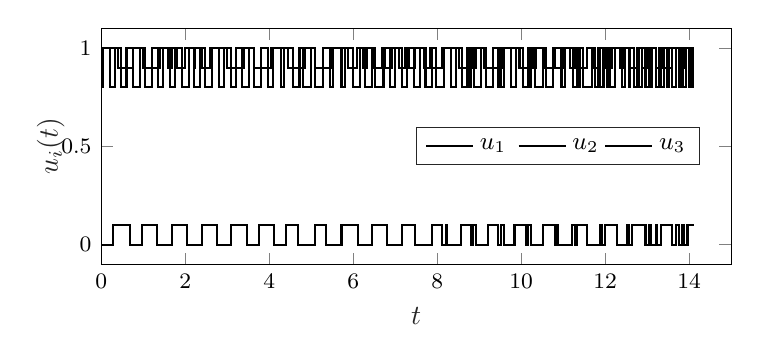
\begin{tikzpicture}

\begin{axis}[%
width=8cm,
height=3cm,
at={(0in,0in)},
scale only axis,
xmin=0.000,
xmax=15.000,
xlabel style={font=\color{white!15!black}},
xlabel={$t$},
ymin=-0.100,
ymax=1.100,
ylabel style={font=\color{white!15!black}, yshift=-8pt},
ylabel={$u_i(t)$},
axis background/.style={fill=white},
legend columns = 3,
legend style={legend cell align=left, font=\small, align=left, draw=white!15!black,
	at={(0.95,0.5)}, anchor=east,
	/tikz/column 2/.style={column sep=0.075cm}},
%legend image post style={line width = 1pt},
every tick label/.append style={font=\footnotesize}
]

\addplot [color=black, line width=0.75pt]
  table[row sep=crcr]{%
0.000	0.000\\
0.280	0.000\\
0.280	0.100\\
0.680	0.100\\
0.680	0.000\\
0.960	0.000\\
0.960	0.100\\
1.320	0.100\\
1.320	0.000\\
1.680	0.000\\
1.680	0.100\\
2.040	0.100\\
2.040	0.000\\
2.400	0.000\\
2.400	0.100\\
2.760	0.100\\
2.760	0.000\\
3.080	0.000\\
3.080	0.100\\
3.480	0.100\\
3.480	0.000\\
3.760	0.000\\
3.760	0.100\\
4.120	0.100\\
4.120	0.000\\
4.400	0.000\\
4.400	0.100\\
4.680	0.100\\
4.680	0.000\\
5.080	0.000\\
5.080	0.100\\
5.360	0.100\\
5.360	0.000\\
5.720	0.000\\
5.720	0.100\\
6.120	0.100\\
6.120	0.000\\
6.440	0.000\\
6.440	0.100\\
6.800	0.100\\
6.800	0.000\\
7.160	0.000\\
7.160	0.100\\
7.480	0.100\\
7.480	0.000\\
7.880	0.000\\
7.880	0.100\\
8.120	0.100\\
8.120	0.000\\
8.200	0.000\\
8.200	0.100\\
8.240	0.100\\
8.240	0.000\\
8.560	0.000\\
8.560	0.100\\
8.800	0.100\\
8.800	0.000\\
8.840	0.000\\
8.840	0.100\\
8.920	0.100\\
8.920	0.000\\
9.200	0.000\\
9.200	0.100\\
9.440	0.100\\
9.440	0.000\\
9.520	0.000\\
9.520	0.100\\
9.600	0.100\\
9.600	0.000\\
9.840	0.000\\
9.840	0.100\\
10.120	0.100\\
10.120	0.000\\
10.160	0.000\\
10.160	0.100\\
10.240	0.100\\
10.240	0.000\\
10.520	0.000\\
10.520	0.100\\
10.800	0.100\\
10.800	0.000\\
10.840	0.000\\
10.840	0.100\\
10.880	0.100\\
10.880	0.000\\
11.200	0.000\\
11.200	0.100\\
11.280	0.100\\
11.280	0.000\\
11.320	0.000\\
11.320	0.100\\
11.560	0.100\\
11.560	0.000\\
11.880	0.000\\
11.880	0.100\\
11.920	0.100\\
11.920	0.000\\
12.000	0.000\\
12.000	0.100\\
12.280	0.100\\
12.280	0.000\\
12.520	0.000\\
12.520	0.100\\
12.560	0.100\\
12.560	0.000\\
12.640	0.000\\
12.640	0.100\\
12.960	0.100\\
12.960	0.000\\
13.040	0.000\\
13.040	0.100\\
13.080	0.100\\
13.080	0.000\\
13.200	0.000\\
13.200	0.100\\
13.240	0.100\\
13.240	0.000\\
13.320	0.000\\
13.320	0.100\\
13.600	0.100\\
13.600	0.000\\
13.680	0.000\\
13.680	0.100\\
13.760	0.100\\
13.760	0.000\\
13.840	0.000\\
13.840	0.100\\
13.880	0.100\\
13.880	0.000\\
13.960	0.000\\
13.960	0.100\\
14.120	0.100\\
};
\addlegendentry{$u_1$}

\addplot [color=black, line width=0.75pt]
  table[row sep=crcr]{%
0.000	0.800\\
0.040	0.800\\
0.040	1.000\\
0.200	1.000\\
0.200	0.800\\
0.320	0.800\\
0.320	1.000\\
0.480	1.000\\
0.480	0.800\\
0.600	0.800\\
0.600	1.000\\
0.760	1.000\\
0.760	0.800\\
0.920	0.800\\
0.920	1.000\\
1.040	1.000\\
1.040	0.800\\
1.200	0.800\\
1.200	1.000\\
1.360	1.000\\
1.360	0.800\\
1.480	0.800\\
1.480	1.000\\
1.640	1.000\\
1.640	0.800\\
1.760	0.800\\
1.760	1.000\\
1.920	1.000\\
1.920	0.800\\
2.080	0.800\\
2.080	1.000\\
2.200	1.000\\
2.200	0.800\\
2.360	0.800\\
2.360	1.000\\
2.480	1.000\\
2.480	0.800\\
2.640	0.800\\
2.640	1.000\\
2.800	1.000\\
2.800	0.800\\
2.920	0.800\\
2.920	1.000\\
3.080	1.000\\
3.080	0.800\\
3.200	0.800\\
3.200	1.000\\
3.360	1.000\\
3.360	0.800\\
3.520	0.800\\
3.520	1.000\\
3.640	1.000\\
3.640	0.800\\
3.800	0.800\\
3.800	1.000\\
3.960	1.000\\
3.960	0.800\\
4.080	0.800\\
4.080	1.000\\
4.280	1.000\\
4.280	0.800\\
4.360	0.800\\
4.360	1.000\\
4.560	1.000\\
4.560	0.800\\
4.720	0.800\\
4.720	1.000\\
4.800	1.000\\
4.800	0.800\\
5.000	0.800\\
5.000	1.000\\
5.080	1.000\\
5.080	0.800\\
5.280	0.800\\
5.280	1.000\\
5.440	1.000\\
5.440	0.800\\
5.520	0.800\\
5.520	1.000\\
5.720	1.000\\
5.720	0.800\\
5.800	0.800\\
5.800	1.000\\
6.000	1.000\\
6.000	0.800\\
6.160	0.800\\
6.160	1.000\\
6.280	1.000\\
6.280	0.800\\
6.440	0.800\\
6.440	1.000\\
6.520	1.000\\
6.520	0.800\\
6.720	0.800\\
6.720	1.000\\
6.880	1.000\\
6.880	0.800\\
7.000	0.800\\
7.000	1.000\\
7.160	1.000\\
7.160	0.800\\
7.280	0.800\\
7.280	1.000\\
7.440	1.000\\
7.440	0.800\\
7.600	0.800\\
7.600	1.000\\
7.720	1.000\\
7.720	0.800\\
7.880	0.800\\
7.880	1.000\\
7.960	1.000\\
7.960	0.800\\
8.160	0.800\\
8.160	1.000\\
8.320	1.000\\
8.320	0.800\\
8.440	0.800\\
8.440	1.000\\
8.600	1.000\\
8.600	0.800\\
8.720	0.800\\
8.720	1.000\\
8.760	1.000\\
8.760	0.800\\
8.800	0.800\\
8.800	1.000\\
8.880	1.000\\
8.880	0.800\\
9.040	0.800\\
9.040	1.000\\
9.160	1.000\\
9.160	0.800\\
9.320	0.800\\
9.320	1.000\\
9.440	1.000\\
9.440	0.800\\
9.480	0.800\\
9.480	1.000\\
9.520	1.000\\
9.520	0.800\\
9.600	0.800\\
9.600	1.000\\
9.760	1.000\\
9.760	0.800\\
9.880	0.800\\
9.880	1.000\\
10.040	1.000\\
10.040	0.800\\
10.160	0.800\\
10.160	1.000\\
10.200	1.000\\
10.200	0.800\\
10.240	0.800\\
10.240	1.000\\
10.320	1.000\\
10.320	0.800\\
10.520	0.800\\
10.520	1.000\\
10.600	1.000\\
10.600	0.800\\
10.760	0.800\\
10.760	1.000\\
10.960	1.000\\
10.960	0.800\\
11.040	0.800\\
11.040	1.000\\
11.240	1.000\\
11.240	0.800\\
11.320	0.800\\
11.320	1.000\\
11.360	1.000\\
11.360	0.800\\
11.400	0.800\\
11.400	1.000\\
11.480	1.000\\
11.480	0.800\\
11.680	0.800\\
11.680	1.000\\
11.760	1.000\\
11.760	0.800\\
11.840	0.800\\
11.840	1.000\\
11.880	1.000\\
11.880	0.800\\
11.960	0.800\\
11.960	1.000\\
12.040	1.000\\
12.040	0.800\\
12.080	0.800\\
12.080	1.000\\
12.120	1.000\\
12.120	0.800\\
12.240	0.800\\
12.240	1.000\\
12.400	1.000\\
12.400	0.800\\
12.480	0.800\\
12.480	1.000\\
12.560	1.000\\
12.560	0.800\\
12.600	0.800\\
12.600	1.000\\
12.680	1.000\\
12.680	0.800\\
12.760	0.800\\
12.760	1.000\\
12.800	1.000\\
12.800	0.800\\
12.880	0.800\\
12.880	1.000\\
12.960	1.000\\
12.960	0.800\\
13.040	0.800\\
13.040	1.000\\
13.080	1.000\\
13.080	0.800\\
13.120	0.800\\
13.120	1.000\\
13.200	1.000\\
13.200	0.800\\
13.280	0.800\\
13.280	1.000\\
13.320	1.000\\
13.320	0.800\\
13.400	0.800\\
13.400	1.000\\
13.480	1.000\\
13.480	0.800\\
13.520	0.800\\
13.520	1.000\\
13.600	1.000\\
13.600	0.800\\
13.680	0.800\\
13.680	1.000\\
13.760	1.000\\
13.760	0.800\\
13.800	0.800\\
13.800	1.000\\
13.840	1.000\\
13.840	0.800\\
13.920	0.800\\
13.920	1.000\\
14.000	1.000\\
14.000	0.800\\
14.040	0.800\\
14.040	1.000\\
14.080	1.000\\
14.080	0.800\\
14.120	0.800\\
};
\addlegendentry{$u_2$}

\addplot [color=black, line width=0.75pt]
  table[row sep=crcr]{%
0.000	1.000\\
0.400	1.000\\
0.400	0.900\\
0.760	0.900\\
0.760	1.000\\
1.000	1.000\\
1.000	0.900\\
1.400	0.900\\
1.400	1.000\\
1.600	1.000\\
1.600	0.900\\
1.680	0.900\\
1.680	1.000\\
1.800	1.000\\
1.800	0.900\\
2.000	0.900\\
2.000	1.000\\
2.200	1.000\\
2.200	0.900\\
2.240	0.900\\
2.240	1.000\\
2.400	1.000\\
2.400	0.900\\
2.600	0.900\\
2.600	1.000\\
3.000	1.000\\
3.000	0.900\\
3.400	0.900\\
3.400	1.000\\
3.640	1.000\\
3.640	0.900\\
4.040	0.900\\
4.040	1.000\\
4.440	1.000\\
4.440	0.900\\
4.840	0.900\\
4.840	1.000\\
5.080	1.000\\
5.080	0.900\\
5.480	0.900\\
5.480	1.000\\
5.880	1.000\\
5.880	0.900\\
6.080	0.900\\
6.080	1.000\\
6.240	1.000\\
6.240	0.900\\
6.320	0.900\\
6.320	1.000\\
6.480	1.000\\
6.480	0.900\\
6.680	0.900\\
6.680	1.000\\
6.760	1.000\\
6.760	0.900\\
6.920	0.900\\
6.920	1.000\\
7.080	1.000\\
7.080	0.900\\
7.240	0.900\\
7.240	1.000\\
7.320	1.000\\
7.320	0.900\\
7.480	0.900\\
7.480	1.000\\
7.680	1.000\\
7.680	0.900\\
7.840	0.900\\
7.840	1.000\\
7.880	1.000\\
7.880	0.900\\
8.120	0.900\\
8.120	1.000\\
8.520	1.000\\
8.520	0.900\\
8.760	0.900\\
8.760	1.000\\
8.840	1.000\\
8.840	0.900\\
8.920	0.900\\
8.920	1.000\\
9.120	1.000\\
9.120	0.900\\
9.560	0.900\\
9.560	1.000\\
9.960	1.000\\
9.960	0.900\\
10.160	0.900\\
10.160	1.000\\
10.280	1.000\\
10.280	0.900\\
10.360	0.900\\
10.360	1.000\\
10.560	1.000\\
10.560	0.900\\
10.760	0.900\\
10.760	1.000\\
10.800	1.000\\
10.800	0.900\\
11.000	0.900\\
11.000	1.000\\
11.160	1.000\\
11.160	0.900\\
11.280	0.900\\
11.280	1.000\\
11.400	1.000\\
11.400	0.900\\
11.560	0.900\\
11.560	1.000\\
11.720	1.000\\
11.720	0.900\\
11.880	0.900\\
11.880	1.000\\
12.000	1.000\\
12.000	0.900\\
12.160	0.900\\
12.160	1.000\\
12.360	1.000\\
12.360	0.900\\
12.440	0.900\\
12.440	1.000\\
12.600	1.000\\
12.600	0.900\\
12.800	0.900\\
12.800	1.000\\
12.880	1.000\\
12.880	0.900\\
13.000	0.900\\
13.000	1.000\\
13.200	1.000\\
13.200	0.900\\
13.360	0.900\\
13.360	1.000\\
13.400	1.000\\
13.400	0.900\\
13.600	0.900\\
13.600	1.000\\
13.840	1.000\\
13.840	0.900\\
13.880	0.900\\
13.880	1.000\\
14.000	1.000\\
14.000	0.900\\
14.120	0.900\\
};
\addlegendentry{$u_3$}

\end{axis}

\end{tikzpicture}
}{
    % This file was created by matlab2tikz.
%
%The latest updates can be retrieved from
%  http://www.mathworks.com/matlabcentral/fileexchange/22022-matlab2tikz-matlab2tikz
%where you can also make suggestions and rate matlab2tikz.
%
\definecolor{mycolor1}{rgb}{0.00000,0.36078,0.67059}%
\definecolor{mycolor2}{rgb}{0.89020,0.10588,0.13725}%

\tikzsetnextfilename{figure_cvd_good}
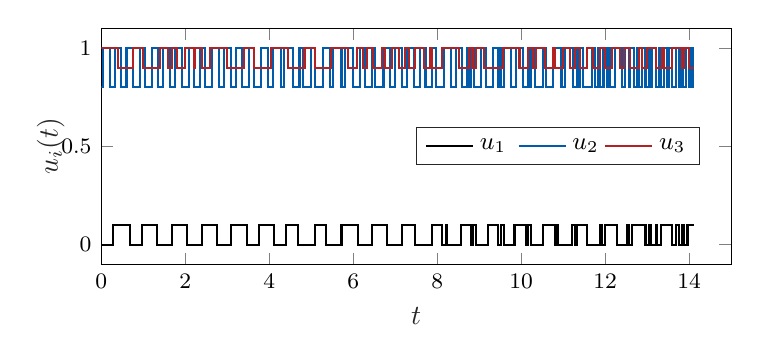
\begin{tikzpicture}

\begin{axis}[%
width=8cm,
height=3cm,
at={(0in,0in)},
scale only axis,
xmin=0.000,
xmax=15.000,
xlabel style={font=\color{white!15!black}},
xlabel={$t$},
ymin=-0.100,
ymax=1.100,
ylabel style={font=\color{white!15!black}, yshift=-8pt},
ylabel={$u_i(t)$},
axis background/.style={fill=white},
legend columns = 3,
legend style={legend cell align=left, font=\small, align=left, draw=white!15!black,
	at={(0.95,0.5)}, anchor=east,
	/tikz/column 2/.style={column sep=0.075cm}},
%legend image post style={line width = 1pt},
every tick label/.append style={font=\footnotesize}
]

\addplot [color=black, line width=0.75pt]
  table[row sep=crcr]{%
0.000	0.000\\
0.280	0.000\\
0.280	0.100\\
0.680	0.100\\
0.680	0.000\\
0.960	0.000\\
0.960	0.100\\
1.320	0.100\\
1.320	0.000\\
1.680	0.000\\
1.680	0.100\\
2.040	0.100\\
2.040	0.000\\
2.400	0.000\\
2.400	0.100\\
2.760	0.100\\
2.760	0.000\\
3.080	0.000\\
3.080	0.100\\
3.480	0.100\\
3.480	0.000\\
3.760	0.000\\
3.760	0.100\\
4.120	0.100\\
4.120	0.000\\
4.400	0.000\\
4.400	0.100\\
4.680	0.100\\
4.680	0.000\\
5.080	0.000\\
5.080	0.100\\
5.360	0.100\\
5.360	0.000\\
5.720	0.000\\
5.720	0.100\\
6.120	0.100\\
6.120	0.000\\
6.440	0.000\\
6.440	0.100\\
6.800	0.100\\
6.800	0.000\\
7.160	0.000\\
7.160	0.100\\
7.480	0.100\\
7.480	0.000\\
7.880	0.000\\
7.880	0.100\\
8.120	0.100\\
8.120	0.000\\
8.200	0.000\\
8.200	0.100\\
8.240	0.100\\
8.240	0.000\\
8.560	0.000\\
8.560	0.100\\
8.800	0.100\\
8.800	0.000\\
8.840	0.000\\
8.840	0.100\\
8.920	0.100\\
8.920	0.000\\
9.200	0.000\\
9.200	0.100\\
9.440	0.100\\
9.440	0.000\\
9.520	0.000\\
9.520	0.100\\
9.600	0.100\\
9.600	0.000\\
9.840	0.000\\
9.840	0.100\\
10.120	0.100\\
10.120	0.000\\
10.160	0.000\\
10.160	0.100\\
10.240	0.100\\
10.240	0.000\\
10.520	0.000\\
10.520	0.100\\
10.800	0.100\\
10.800	0.000\\
10.840	0.000\\
10.840	0.100\\
10.880	0.100\\
10.880	0.000\\
11.200	0.000\\
11.200	0.100\\
11.280	0.100\\
11.280	0.000\\
11.320	0.000\\
11.320	0.100\\
11.560	0.100\\
11.560	0.000\\
11.880	0.000\\
11.880	0.100\\
11.920	0.100\\
11.920	0.000\\
12.000	0.000\\
12.000	0.100\\
12.280	0.100\\
12.280	0.000\\
12.520	0.000\\
12.520	0.100\\
12.560	0.100\\
12.560	0.000\\
12.640	0.000\\
12.640	0.100\\
12.960	0.100\\
12.960	0.000\\
13.040	0.000\\
13.040	0.100\\
13.080	0.100\\
13.080	0.000\\
13.200	0.000\\
13.200	0.100\\
13.240	0.100\\
13.240	0.000\\
13.320	0.000\\
13.320	0.100\\
13.600	0.100\\
13.600	0.000\\
13.680	0.000\\
13.680	0.100\\
13.760	0.100\\
13.760	0.000\\
13.840	0.000\\
13.840	0.100\\
13.880	0.100\\
13.880	0.000\\
13.960	0.000\\
13.960	0.100\\
14.120	0.100\\
};
\addlegendentry{$u_1$}

\addplot [color=color_guideline, line width=0.75pt]
  table[row sep=crcr]{%
0.000	0.800\\
0.040	0.800\\
0.040	1.000\\
0.200	1.000\\
0.200	0.800\\
0.320	0.800\\
0.320	1.000\\
0.480	1.000\\
0.480	0.800\\
0.600	0.800\\
0.600	1.000\\
0.760	1.000\\
0.760	0.800\\
0.920	0.800\\
0.920	1.000\\
1.040	1.000\\
1.040	0.800\\
1.200	0.800\\
1.200	1.000\\
1.360	1.000\\
1.360	0.800\\
1.480	0.800\\
1.480	1.000\\
1.640	1.000\\
1.640	0.800\\
1.760	0.800\\
1.760	1.000\\
1.920	1.000\\
1.920	0.800\\
2.080	0.800\\
2.080	1.000\\
2.200	1.000\\
2.200	0.800\\
2.360	0.800\\
2.360	1.000\\
2.480	1.000\\
2.480	0.800\\
2.640	0.800\\
2.640	1.000\\
2.800	1.000\\
2.800	0.800\\
2.920	0.800\\
2.920	1.000\\
3.080	1.000\\
3.080	0.800\\
3.200	0.800\\
3.200	1.000\\
3.360	1.000\\
3.360	0.800\\
3.520	0.800\\
3.520	1.000\\
3.640	1.000\\
3.640	0.800\\
3.800	0.800\\
3.800	1.000\\
3.960	1.000\\
3.960	0.800\\
4.080	0.800\\
4.080	1.000\\
4.280	1.000\\
4.280	0.800\\
4.360	0.800\\
4.360	1.000\\
4.560	1.000\\
4.560	0.800\\
4.720	0.800\\
4.720	1.000\\
4.800	1.000\\
4.800	0.800\\
5.000	0.800\\
5.000	1.000\\
5.080	1.000\\
5.080	0.800\\
5.280	0.800\\
5.280	1.000\\
5.440	1.000\\
5.440	0.800\\
5.520	0.800\\
5.520	1.000\\
5.720	1.000\\
5.720	0.800\\
5.800	0.800\\
5.800	1.000\\
6.000	1.000\\
6.000	0.800\\
6.160	0.800\\
6.160	1.000\\
6.280	1.000\\
6.280	0.800\\
6.440	0.800\\
6.440	1.000\\
6.520	1.000\\
6.520	0.800\\
6.720	0.800\\
6.720	1.000\\
6.880	1.000\\
6.880	0.800\\
7.000	0.800\\
7.000	1.000\\
7.160	1.000\\
7.160	0.800\\
7.280	0.800\\
7.280	1.000\\
7.440	1.000\\
7.440	0.800\\
7.600	0.800\\
7.600	1.000\\
7.720	1.000\\
7.720	0.800\\
7.880	0.800\\
7.880	1.000\\
7.960	1.000\\
7.960	0.800\\
8.160	0.800\\
8.160	1.000\\
8.320	1.000\\
8.320	0.800\\
8.440	0.800\\
8.440	1.000\\
8.600	1.000\\
8.600	0.800\\
8.720	0.800\\
8.720	1.000\\
8.760	1.000\\
8.760	0.800\\
8.800	0.800\\
8.800	1.000\\
8.880	1.000\\
8.880	0.800\\
9.040	0.800\\
9.040	1.000\\
9.160	1.000\\
9.160	0.800\\
9.320	0.800\\
9.320	1.000\\
9.440	1.000\\
9.440	0.800\\
9.480	0.800\\
9.480	1.000\\
9.520	1.000\\
9.520	0.800\\
9.600	0.800\\
9.600	1.000\\
9.760	1.000\\
9.760	0.800\\
9.880	0.800\\
9.880	1.000\\
10.040	1.000\\
10.040	0.800\\
10.160	0.800\\
10.160	1.000\\
10.200	1.000\\
10.200	0.800\\
10.240	0.800\\
10.240	1.000\\
10.320	1.000\\
10.320	0.800\\
10.520	0.800\\
10.520	1.000\\
10.600	1.000\\
10.600	0.800\\
10.760	0.800\\
10.760	1.000\\
10.960	1.000\\
10.960	0.800\\
11.040	0.800\\
11.040	1.000\\
11.240	1.000\\
11.240	0.800\\
11.320	0.800\\
11.320	1.000\\
11.360	1.000\\
11.360	0.800\\
11.400	0.800\\
11.400	1.000\\
11.480	1.000\\
11.480	0.800\\
11.680	0.800\\
11.680	1.000\\
11.760	1.000\\
11.760	0.800\\
11.840	0.800\\
11.840	1.000\\
11.880	1.000\\
11.880	0.800\\
11.960	0.800\\
11.960	1.000\\
12.040	1.000\\
12.040	0.800\\
12.080	0.800\\
12.080	1.000\\
12.120	1.000\\
12.120	0.800\\
12.240	0.800\\
12.240	1.000\\
12.400	1.000\\
12.400	0.800\\
12.480	0.800\\
12.480	1.000\\
12.560	1.000\\
12.560	0.800\\
12.600	0.800\\
12.600	1.000\\
12.680	1.000\\
12.680	0.800\\
12.760	0.800\\
12.760	1.000\\
12.800	1.000\\
12.800	0.800\\
12.880	0.800\\
12.880	1.000\\
12.960	1.000\\
12.960	0.800\\
13.040	0.800\\
13.040	1.000\\
13.080	1.000\\
13.080	0.800\\
13.120	0.800\\
13.120	1.000\\
13.200	1.000\\
13.200	0.800\\
13.280	0.800\\
13.280	1.000\\
13.320	1.000\\
13.320	0.800\\
13.400	0.800\\
13.400	1.000\\
13.480	1.000\\
13.480	0.800\\
13.520	0.800\\
13.520	1.000\\
13.600	1.000\\
13.600	0.800\\
13.680	0.800\\
13.680	1.000\\
13.760	1.000\\
13.760	0.800\\
13.800	0.800\\
13.800	1.000\\
13.840	1.000\\
13.840	0.800\\
13.920	0.800\\
13.920	1.000\\
14.000	1.000\\
14.000	0.800\\
14.040	0.800\\
14.040	1.000\\
14.080	1.000\\
14.080	0.800\\
14.120	0.800\\
};
\addlegendentry{$u_2$}

\addplot [color=color_example_bad, line width=0.75pt]
  table[row sep=crcr]{%
0.000	1.000\\
0.400	1.000\\
0.400	0.900\\
0.760	0.900\\
0.760	1.000\\
1.000	1.000\\
1.000	0.900\\
1.400	0.900\\
1.400	1.000\\
1.600	1.000\\
1.600	0.900\\
1.680	0.900\\
1.680	1.000\\
1.800	1.000\\
1.800	0.900\\
2.000	0.900\\
2.000	1.000\\
2.200	1.000\\
2.200	0.900\\
2.240	0.900\\
2.240	1.000\\
2.400	1.000\\
2.400	0.900\\
2.600	0.900\\
2.600	1.000\\
3.000	1.000\\
3.000	0.900\\
3.400	0.900\\
3.400	1.000\\
3.640	1.000\\
3.640	0.900\\
4.040	0.900\\
4.040	1.000\\
4.440	1.000\\
4.440	0.900\\
4.840	0.900\\
4.840	1.000\\
5.080	1.000\\
5.080	0.900\\
5.480	0.900\\
5.480	1.000\\
5.880	1.000\\
5.880	0.900\\
6.080	0.900\\
6.080	1.000\\
6.240	1.000\\
6.240	0.900\\
6.320	0.900\\
6.320	1.000\\
6.480	1.000\\
6.480	0.900\\
6.680	0.900\\
6.680	1.000\\
6.760	1.000\\
6.760	0.900\\
6.920	0.900\\
6.920	1.000\\
7.080	1.000\\
7.080	0.900\\
7.240	0.900\\
7.240	1.000\\
7.320	1.000\\
7.320	0.900\\
7.480	0.900\\
7.480	1.000\\
7.680	1.000\\
7.680	0.900\\
7.840	0.900\\
7.840	1.000\\
7.880	1.000\\
7.880	0.900\\
8.120	0.900\\
8.120	1.000\\
8.520	1.000\\
8.520	0.900\\
8.760	0.900\\
8.760	1.000\\
8.840	1.000\\
8.840	0.900\\
8.920	0.900\\
8.920	1.000\\
9.120	1.000\\
9.120	0.900\\
9.560	0.900\\
9.560	1.000\\
9.960	1.000\\
9.960	0.900\\
10.160	0.900\\
10.160	1.000\\
10.280	1.000\\
10.280	0.900\\
10.360	0.900\\
10.360	1.000\\
10.560	1.000\\
10.560	0.900\\
10.760	0.900\\
10.760	1.000\\
10.800	1.000\\
10.800	0.900\\
11.000	0.900\\
11.000	1.000\\
11.160	1.000\\
11.160	0.900\\
11.280	0.900\\
11.280	1.000\\
11.400	1.000\\
11.400	0.900\\
11.560	0.900\\
11.560	1.000\\
11.720	1.000\\
11.720	0.900\\
11.880	0.900\\
11.880	1.000\\
12.000	1.000\\
12.000	0.900\\
12.160	0.900\\
12.160	1.000\\
12.360	1.000\\
12.360	0.900\\
12.440	0.900\\
12.440	1.000\\
12.600	1.000\\
12.600	0.900\\
12.800	0.900\\
12.800	1.000\\
12.880	1.000\\
12.880	0.900\\
13.000	0.900\\
13.000	1.000\\
13.200	1.000\\
13.200	0.900\\
13.360	0.900\\
13.360	1.000\\
13.400	1.000\\
13.400	0.900\\
13.600	0.900\\
13.600	1.000\\
13.840	1.000\\
13.840	0.900\\
13.880	0.900\\
13.880	1.000\\
14.000	1.000\\
14.000	0.900\\
14.120	0.900\\
};
\addlegendentry{$u_3$}

\end{axis}

\end{tikzpicture}
}

\noindent
Color vision deficiency affects approximately $8\%$ of men and $0.5\%$ of women worldwide, or roughly $1$ in $12$ men and $1$ in $200$ women \footfullcite{Gordon1998}.
As a result, it is highly likely that some readers would benefit from color choices that accommodate this condition.
The ``bad'' version in the example above uses only black lines to simulate how indistinguishable colors can appear to individuals with color vision deficiency.


\guideline[g:nontext:figure_linestyles]
    {Figures: Consider using different line styles.}

\goodbadexample{
    ...
}{
    ...
}

\noindent Varying line styles help differentiate information, making figures more accessible and easier to interpret.
Additionally, line styles are easier to reference in the caption, as colors may appear differently in black-and-white prints.


\guideline[g:nontext:figure_caption]
    {Figures: Captions should provide a brief, independent summary.}

% bad: caption that does not fully explain what is going on
% note: some parts may be explained by the legend, too
\goodbadexample{
    ...
}{
    ...
}

\noindent A good caption provides a concise description of the figure's content, enabling it to be understood without reference to the running text.
To achieve this, all objects, lines, and shading should be clearly explained.

% tables

\guideline[g:nontext:table_horizontal_lines]
    {Tables: Avoid horizontal lines.}

\goodbadexample{
    ...
}{
    ...
}

\noindent Excessive use of horizontal lines can make a table look cluttered and hinder the reader's ability to quickly scan and interpret the data, as the structure provided by rows and columns is often enough to visually separate data.
Horizontal lines are primarily used for sectioning, e.g., between column headers and data, or between different segments of similar data.


\guideline{Tables: Highlight the best values in bold when comparing results.}

\goodbadexample{
    ...
}{
    ...
}

\noindent Highlighting the best values adds a layer of visual hierarchy to the table, helping readers more easily compare data.
This can also support arguments about the quality of the results, as multiple bold entries suggest strong performance.


\guideline[g:nontext:table_caption]
    {Tables: Explain all variables used in the caption.}

\goodbadexample{
    ...
}{
    ...
}

\noindent To enable readers to understand the table independently of the running text, the caption should concisely describe all variables used, even if their meaning is consistent throughout the paper.
This explanation usually comes after a brief summary of the table's content.

% pseudocode

\guideline[g:nontext:pseudocode_language_specific]
    {Avoid language-specific functions in pseudocode.}

\goodbadexample{
    \textbf{Algorithm 1.} A good algorithm. \\
    Input: Matrix $G$, (...) \\
    Output: (...) \\
    \begin{scriptsize}
        1:
    \end{scriptsize}
    $m \gets \highlightpartmath{\textsc{shape}(G,2)}$ \\
    (...)
}{
    \textbf{Algorithm 1.} A good algorithm. \\
    Input: Matrix $G \in \mathbb{R}^{n \times \highlightpartmath{m}}$, (...) \\
    Output: (...) \\
    (...)
}

\noindent Using language-specific functions may hinder understanding across diverse audiences, as some readers may not be familiar with any given programming language.
In simple cases, there may be a more rigorous way to achieve the same goal, as shown in the example above.
If a language-specific function is particularly useful, its behavior can be briefly described in the running text.


\guideline[g:nontext:pseudocode_explain_operators]
    {Pseudocode: Ensure that all operators are explained or referenced.}

\goodbadexample{
    ...
}{
    ...
}

\noindent Since pseudocode aims to be concise, it's often better to use named operations rather than detailing every computation, especially for standard tasks, e.g., sorting.
However, it is still good practice to briefly explain what each operation does, particularly in terms of its input and output arguments.


\guideline[g:nontext:pseudocode_io_arguments]
    {Pseudocode: Strictly define the input and output arguments.}

% use a short pseudocode...
\goodexample{
    ...
}

\noindent A clear definition of input and output arguments integrates these variables more seamlessly into the surrounding text and facilitates cross-referencing between sections.
It also helps those re-implementing a specific pseudocode.


\chapter{Wording}
\label{ch:wording}

Correct wording is crucial to ensure the clear communication of the scientific content.
The following guidelines help refine sentences to enhance the overall readability of their work.


\guideline{Introduce abbreviations at their earliest occurrence, use only the abbreviation afterward.}

\goodexample{
    Platooning is often realized via \highlightpart{Cooperative Adaptive Cruise Control (CACC)}: longitudinal vehicle control that incorporates information from inter-vehicle communication.
    (...)
    Our proposed safety concept is agnostic of the underlying \highlightpart{CACC}.
}

\noindent Please note that the abstract is not part of the main body and, therefore, does not constitute the first occurrence.


\guideline{Prefer active voice over passive voice.}

\goodbadexample{
    This \highlightpart{is realized by} explicitly preserving the non-convex dependencies of all involved variables through all layers of the graph neural network using polynomial zonotopes.
}{
    \highlightpart{We use} polynomial zonotopes to explicitly preserve the non-convex dependencies of all invovled variables through all layers of the graph neural network.
}

\noindent Active voice is usually clearer and more concise, as the subject-verb-object structure is easy to follow, emphasizes the action, and requires fewer words.
The frequency of using passive voice is often influenced by the author's native language.


\guideline[g:wording:address_reader_imperative]
    {Address the reader by imperatives only.}

\goodbadexample[{\cite[Sec.~IV]{Wetzlinger2024CSL}}]{
    \highlightpart{You will notice} that the number of steps linearly influences the time complexity.
}{
    \highlightpart{Please note} that the number of steps linearly influences the time complexity.
}

\noindent The most common occurrences are ``consider'' and ``note''.
Alternatively, one can write ``let us (...)''.


\guideline[g:wording:consistent_terms]
    {Use terms consistently.}

\goodbadexample[{\cite[Sec.~I.]{Wetzlinger2024CSL}}]{
    Most approaches for computing \highlightpart{inner approximations} for nonlinear systems are based on outer approximations. 
    (...)
    One can also obtain \highlightpart{under approximations} via optimization-based techniques.
}{
    Most approaches for computing \highlightpart{inner approximations} for nonlinear systems are based on outer approximations.
    (...)
    One can also obtain \highlightpart{inner approximations} via optimization-based techniques.
}

\noindent Consistency in terminology is crucial for ensuring the clarity of the presentation.
Different terms typically imply different meanings, so using them can lead readers to assume a distinction.
Inconsistent use of key terms indicates either uncertainty about the content or, at the very least, a lack of effort to refine the work.


\guideline{Use explicit destinations when referring to other sections.}

\goodbadexample{
    As mentioned \highlightpart{above}, we consider disturbances modeled by probability density functions.
}{
    As mentioned \highlightpart{in Section II-A.}, we consider disturbances modeled by probability density functions.
}

\noindent Clearly specifying the intended section (or structural element) assists the reader in forming an internal map of how different parts of the paper are interconnected;
the narrower the scope of the reference, the better.


\guideline[g:wording:less_fewer]
    {Use ``less'' for uncountable amounts and ``fewer'' for countable amounts.}

\goodbadexample{
    Furthermore, our optimization algorithm converges in \highlightpart{less} steps than state-of-the-art approaches.
}{
    Furthermore, our optimization algorithm converges in \highlightpart{fewer} steps than state-of-the-art approaches.
}

\noindent Paying attention to this distinction is a simple but effective way to improve the clarity of the presentation.


\guideline[g:wording:genitives]
    {Prefer prepositional genitives over possessive genitives.}

\goodbadexample{
    This \highlightpart{approach’s main downside} is that it either only reflects simple linear reward functions or requires thousands of human queries.
}{
    The \highlightpart{main downside of this approach} is that it either only reflects simple linear reward functions or requires thousands of human queries.
}

\noindent Descriptions often address abstract concepts where a possessive relationship is less suitable because the "owner" is inanimate.
Furthermore, prepositional genitives offer more flexibility and better express associative relationships, as is often the case.
One notable exception to this guideline is proper nouns.


\guideline[g:wording:contractions]{Avoid contractions.}

\goodbadexample[{\cite[Sec.~IV.C.]{Wetzlinger2023TAC}}]{
    By successively halving the time step size, \highlightpart{we'll} always find a time step size so that the error bound is satisfied.
}{
    By successively halving the time step size, \highlightpart{we will} always find a time step size so that the error bound is satisfied.
}

\noindent No exceptions.


\guideline[g:wording:it]
    {Avoid using ``it'' as an object.}

\goodbadexample{
    On the other hand, \highlightpart{computing it} with polynomial zonotopes yields (...)
}{
    On the other hand, \highlightpart{evaluating (1)} with polynomial zonotopes yields (...)
}
% TODO: Find a different example...

\noindent Using ``it'' as an object may lead to vagueness (even if it refers to a term mentioned directly beforehand), and there often is a more direct formulation.



\guideline[g:wording:environment_names]
    {Refer to environments instead of introducing new names.}

\goodbadexample[{\cite[Sec.~IV.D.]{Wetzlinger2023TAC}}]{
    \textbf{Algorithm 2.} \highlightpart{\textsc{AutomatedReach}} \\
    (...) \smallskip

    While \highlightpart{\textsc{AutomatedReach}} is guaranteed to converge, there is still room for improvement regarding the computation time.
}{
    \textbf{Algorithm 2.} \highlightpart{Reachability algorithm (automated tuning).} \\
    (...) \smallskip

    While \highlightpart{Algorithm 2} is guaranteed to converge, there is still room for improvement regarding the computation time.
}

\noindent The environment's name serves as an identifier, eliminating the need for an additional one.
Such identifiers seamlessly integrate into running text, as well as pseudocode and tables.


\guideline[g:wording:colloquial_passive]
    {Avoid colloquial passive voice using ``get''.}

\goodbadexample{
    The first approach enforces that the uncertainty sets cannot \highlightpart{get smaller} during the identification process.
}{
    The first approach enforces that the size of the uncertainty sets cannot \highlightpart{decrease} during the identification process.
}

\noindent There always exists a preferable alternative to colloquial passive structures.


\guideline{Avoid explicitly referring to references for details.}

\goodbadexample{
    \textbf{Definition 1} (Model Predictive Robustness [1, Def. 2])
    \textit{The model predictive robustness $\rho_p \in [-1, 1]$ quantifies the likelihood that the satisfaction or violation status of a predicate $p$ remains consistent over a finite prediction horizon.
    The robustness is assigned a positive sign if the predicate is satisfied, and a negative sign if it is violated.}

    \highlightpart{For a detailed formal definition of model predictive robustness, we refer the reader to [1].}
}{
    \textbf{Definition 1} (Model Predictive Robustness [1, Def. 2])
    \textit{The model predictive robustness $\rho_p \in [-1, 1]$ quantifies the likelihood that the satisfaction or violation status of a predicate $p$ remains consistent over a finite prediction horizon.
    The robustness is assigned a positive sign if the predicate is satisfied, and a negative sign if it is violated.}

    \highlightempty{}
}

\noindent The additional sentence adds no new information, as reference $[1]$ is already included in the definition.
Readers are not expected to see all details repeated, only those the author deems relevant.
Moreover, they know to consult references for further details, as this is a primary purpose of citations.


\guideline[g:wording:long_sentences]
    {Avoid overly long sentences.}

\goodbadexample[{\cite[Sec.~IV.B.]{Wetzlinger2025TAC}}]{
    As a wide range of different yet similar definitions are labeled \textit{backward reachable set}, the following literature review discusses the various types in order of increasing complexity, in discrete and continuous time as well as for linear and nonlinear dynamics, where uniqueness of solution trajectories and sufficient differentiability are assumed.
}{
    A wide range of different yet similar definitions are labeled \textit{backward reachable set}\highlightpart{.}
    The following literature review introduces the various types in order of increasing complexity\highlightpart{.}
    We discuss approaches in discrete and continuous time as well as for linear and nonlinear dynamics, where uniqueness of solution trajectories and sufficient differentiability are assumed.
}

\noindent As a simple rule of thumb, four lines in double-column format is a suitable threshold to determine whether a sentence is too long.
This threshold is less rigid in case of lengthy terms such as ``backward reachability analysis of nonlinear systems''.
One may also use the number of clauses as a metric to decide whether a sentence should be split in two sentences.
Finally, one can also read a sentence out loud and decide whether it is digestible.


\guideline[g:wording:succinct_formulations]
    {Prefer succinct formulations of verbose ones.}

\goodbadexample{
    Therefore, in our previous work [1]--[5], we \highlightpart{delve into the selection} of the branching point \highlightpart{in a sophisticated way} using criticality measures [6].
}{
    Therefore, in our previous work [1]--[5], we \highlightpart{selected branching points} using criticality measures [6].
}

\noindent Given the length and density of scientific works, it is better to provide clear and concise formulations that accommodate the reader, avoiding unnecessary complexity through verbosity.


\guideline{Use ``that'' for necessary details and ``which'' for supplementary details.}

\goodbadexample{
    For this analysis, we require system models\highlightpart{, which} are able to represent the behavior of the corresponding real system.
}{
    For this analysis, we require system models \highlightpart{that} are able to represent the behavior of the corresponding real system.
}

\goodbadexample{
    One of the main techniques to provide safety guarantees is reachability analysis \highlightpart{that} predicts all possible future system behaviors under uncertainty in the initial state
    and input.
}{
    One of the main techniques to provide safety guarantees is reachability analysis\highlightpart{,} which predicts all possible future system behaviors under uncertainty in the initial state
    and input.
}

\noindent As a test, one can try removing the clause starting with ``that'' or ``which'' and check whether the sentence remains complete.
The commas are determined by their usage:
The conjunction ``that'' is used in restrictive clauses, which require no comma, whereas ``which'' is used in non-restrictive clauses, which require a comma.


\chapter{Math}
\label{ch:math}

The correct use of mathematics is essential for presenting scientific content clearly and concisely.
Unambiguous notation, precise definitions, and consistent formatting are key to ensuring the material is understandable to a broad audience.


\guideline{Prefer strict notation.}

\goodbadexample{
    We linearize the system at each time step $k \in \{0,...,\highlightpartmath{K}\}$ obtain the sequence of state matrices $A_0, ..., \highlightpartmath{A_K}$.
}{
    \highlightpart{We denote scalars by lowercase letters and matrices by uppercase letters.} \\
    (...) \\
    We linearize the system at each time step $k \in \{0,...,\highlightpartmath{\omega}\}$ obtain the sequence of state matrices $A_0, ..., \highlightpartmath{A_\omega}$.
}

\noindent Stricter notation benefits readers by providing a consistent framework that aids navigation across sections and supports pattern recognition by highlighting subtle differences, which ultimately speeds up comprehension.


\guideline[g:math:footnotes_after_variables]
    {Avoid placing footnote marks after variables.}

\goodbadexample[{\cite[Sec.~4.1]{Wetzlinger2024ARCH2}}]{
    (...) which implements the Quickhull algorithm [20] to efficiently check the redundancy of each point, with a polynomial complexity of $\mathcal{O}(\frac{m}{r} f_r)$\highlightpart{\textsuperscript{2}} with respect to (...) \\
    \smallskip
    \begin{footnotesize}% <-- important!
    \textsuperscript{2}Please note that the conditions for balanced execution [20, Def. 3.1] must hold.
    \end{footnotesize}
}{
    (...) which implements the Quickhull algorithm [20] to efficiently check the redundancy of each point, with a polynomial complexity\highlightpart{\textsuperscript{2}} of $\mathcal{O}(\frac{m}{r} f_r)$ with respect to (...) \\
    \smallskip
    \begin{footnotesize}% <-- important!
    \textsuperscript{2}Please note that the conditions for balanced execution [20, Def. 3.1] must hold.
    \end{footnotesize}
}

\noindent Importantly, footnote marks can be confused with exponentiation.
Although this may sometimes not be a mathematical issue, it is still visually misleading.


\guideline{Use separate environments for complex expressions.}

\goodbadexample{
    Finally, we multiply both sides of $P_k$ with \highlightpart{$T = \text{diag}(I_{n_x+1}, I_{n_w}, \lambda_p^{-1}, I_{n_x} , I_{n_x+1}, I_{n_x} , I_{n_u}, \lambda_w, I_{n_q})$} to obtain the LMI $T^\top P_k T \succeq 0$, which yields the claim.
}{
    Finally, we multiply both sides of $P_k$ with the matrix
    \begin{equation*}
        \text{\highlightpart{$T = \text{diag}(I_{n_x+1}, I_{n_w}, \lambda_p^{-1}, I_{n_x} , I_{n_x+1}, I_{n_x} , I_{n_u}, \lambda_w, I_{n_q})$}}
    \end{equation*}
    to obtain the LMI $T^\top P_k T \succeq 0$, which yields the claim.
}

\noindent The length of the expression and its height (due to subscripts, superscripts, fractions, etc.) can serve as an indicator for the complexity of the expression.
Furthermore, the spacing may be affected if expressions exceed the vertical and horizontal bounds of the line.


\guideline{Introduce variables with a name and a domain.}

\goodbadexample{
    Given an \highlightpart{initial state} \highlightpart{$x_0 = x(t_0)$}, and an \highlightpart{input trajectory} \highlightpart{$u$}, we denote the solution at time $t \geq t_0$ of a system of the form (1) by $\xi(t; x_0, u(\cdot))$.
}{
    Given an \highlightpart{initial state} $x_0$ \highlightpart{$\in \mathbb{R}^n$} at the \highlightpart{initial time} $t_0$ \highlightpart{$\in \mathbb{R}$}, and an \highlightpart{input trajectory} $u$\highlightpart{$\colon \mathbb{R} \to \mathbb{R}^m$}, we denote the solution at time $t \geq t_0$ of a system of the form (1) by $\xi(t; x_0, u(\cdot))$.
}

\noindent Explicitly mentioning the name and the domain is helpful because it prevents misunderstandings, especially for readers who may not be familiar with certain conventions or who may follow different ones.
The introduction of variables including a domain is of particular importance in definitions.
New variables in non-inlined equations should be introduced before or immediately after the equation environment.


\guideline[g:math:no_eq_in_text]
    {Avoid referring to equations with ``Eq.''.}

\goodbadexample[{\cite[Sec.~IV.B.]{Wetzlinger2024CSL}}]{
    In each time step $k \in \{0,...,\omega-1\}$, we first compute a Taylor expansion of the nonlinear dynamics \highlightpart{in eq.~(4)} to obtain the affine dynamics \highlightpart{in eq.~(5)}.
}{
    In each time step $k \in \{0,...,\omega-1\}$, we first compute a Taylor expansion of the nonlinear dynamics \highlightpart{(4)} to obtain the affine dynamics \highlightpart{(5)}.
}

\noindent Numbers in between parentheses should be exclusively used for equation numbering.
By consequence, any such identifier is unique and does not require the prefix ``equation'' or ``eq.''.
Note that some publishers may require the usage of ``eq.'' when citing specific equations from the literature.


\guideline{Use time/space complexities with explicit dependencies.}

\goodbadexample{
    Finally, we prove that our algorithm has \highlightpart{polynomial time complexity}.
}{
    Finally, we prove that the \highlightpart{time complexity} of our algorithm is \highlightpart{polynomial in the state dimension $n$}.
}

\noindent Often, the time/space complexity may be inferred from context.
However, the statement is incomplete without mentioning the variable with respect to which a certain behavior is exhibited.
This is particularly useful for readers who are skimming the text for this specific information.


\guideline[g:math:variable_indices]
    {Use italics for variable indices/superscripts and roman font for indices/superscripts that abbreviate words.}

\goodexample{
    Our adaptive cruise control operates with a planning period of $t$\highlightpart{$_{\text{p}}$}, i.e., it provides a new input at discrete planning times $t$\highlightpart{$_k$} $= k \Delta t$\highlightpart{$_{\text{p}}$} to be applied in the time interval $[t$\highlightpart{$_k$}$, t$\highlightpart{$_{k+1}$}$)$.
}

\noindent In the example above, the index ``p'' refers to the term ``planning period'' and is written in roman font.
In contrast, the index ``k'' refers to the variable time step $k$ and is written in italics.


\guideline[g:math:variable_name]
    {Use variables along with their name, unless the variable is repeated multiple times within the same paragraph.}

\goodbadexample[{\cite[Sec.~III.B.]{Wetzlinger2024CSL}}]{
    Each $\highlightpartmath{x(\Delta t) \in \mathcal{R}(\Delta t)}$ can be expressed using $\highlightpartmath{x(0) \in \mathcal{X}_0}$ and a $\highlightpartmath{z(x(0)) \in \widehat{\mathcal{R}}(\mathcal{L}(\mathcal{R}(\tau_0)))}$ that may depend on \highlightpart{$x(0)$}:
}{
    Each \highlightpart{successor state $x(\Delta t) \in \mathcal{R}(\Delta t)$} can be expressed using an \highlightpart{initial state $x(0) \in \mathcal{X}_0$} and an \highlightpart{error vector $z(x(0)) \in \widehat{\mathcal{R}}(\mathcal{L}(\mathcal{R}(\tau_0)))$} that may depend on \highlightpart{$x(0)$}:
}

\noindent Repeating the name of the variable enhances the fluidity of the running text, as the name conveys much more meaning than the variable alone.
Even more so, as one usually thinks of the meaning of a variable when reading it---which is precisely the name.
If the name has been mentioned recently (in the same sentence, the same paragraph, or within an explanation that spans several paragraphs but outlines a single concept), one can expect the reader to remember it and therefore omit the name.



\chapter{References}
\label{ch:references}

References are primarily used in the introduction and related work sections.
The following guidelines help to avoid common pitfalls when citing existing research.


\guideline{Put citation numbers at the end of clauses.}

\goodbadexample{
    Furthermore, several automated time step adaptation strategies have been developed for guaranteed integration methods \highlightpart{[1--3]} that enclose only a single trajectory rather than a set of trajectories.
}{
    Furthermore, several automated time step adaptation strategies have been developed for guaranteed integration methods that enclose only a single trajectory rather than a set of trajectories \highlightpart{[1--3]}.
}

\noindent In certain cases, a sentence may contain multiple ideas in succession, making it difficult to place references at the end. In such instances, it is necessary to identify a suitable point within the sentence where the reference can be inserted with minimal disruption to the flow.


\guideline[g:references:citation_numbers_as_nouns]
    {Avoid using citation numbers as nouns.}

\goodbadexample[{\cite[Sec.~I.A.]{Wetzlinger2023TAC}}]{
    \highlightpart{In [40]}, the reachable set are recomputed from scratch, where the parameter values are refined using fixed scaling factors after each run.
}{
    \highlightpart{A rather brute-force method proposes to recompute the reachable set from scratch}, where the parameter values are refined using fixed scaling factors after each run \highlightpart{[40]}.
}

\noindent
The use of bits like ``the work in [1]'' or ``the authors in [2]'' does not add any value to the sentence, and is, therefore, redundant.
Any sentence should be readable while skipping the citation numbers, as if they were footnotes.
By consequence, the content is presented more compactly, and the text reads more fluidly.


\guideline[g:references:in_environment_title]
    {Cite the reference in the title of environments.}

\goodbadexample[{\cite[Definition 3]{Wetzlinger2025TAC}}]{
    Next, we introduce zonotopes \highlightpart{[8, Def. 1]}. \\
    \textit{Definition 3 (Zonotope):}
    Given a center $c \in \mathbb{R}^n$ and $\gamma \in \mathbb{N}$ generators stored in the columns in the generator matrix $G \in \mathbb{R}^{n \times \gamma}$, a zonotope $\mathcal{Z} \subset \mathbb{R}^n$ is
    \begin{equation*}
        \mathcal{Z} \coloneqq \bigg\{ c + \sum_{i=1}^{\gamma} G_{(\cdot,i)} \alpha_i \, \Big| \, \alpha_i \in [-1,1] \bigg\} .
    \end{equation*}
    We use the shorthand $\mathcal{Z} = \langle c, G \rangle_Z$.
}{
    Next, we introduce zonotopes. \\
    \textit{Definition 3 (Zonotope \highlightpart{[8, Def. 1]}):}
    Given a center $c \in \mathbb{R}^n$ and $\gamma \in \mathbb{N}$ generators stored in the columns in the generator matrix $G \in \mathbb{R}^{n \times \gamma}$, a zonotope $\mathcal{Z} \subset \mathbb{R}^n$ is
    \begin{equation*}
        \mathcal{Z} \coloneqq \bigg\{ c + \sum_{i=1}^{\gamma} G_{(\cdot,i)} \alpha_i \, \Big| \, \alpha_i \in [-1,1] \bigg\} .
    \end{equation*}
    We use the shorthand $\mathcal{Z} = \langle c, G \rangle_Z$.
}

\noindent
Environments stand out from the surrounding text, which comes with the expectation of self-contained information.
Hence, the reference is better positioned within the environment than before or after.


\guideline[g:references:no_quotes]
    {Do not use direct quotes.}

\goodbadexample{
    ...
}{
    ...
}

\noindent ...


\guideline{Avoid mentioning authors by name.}

\goodbadexample{
    To reduce the computational burden of optimizing affine feedback policies online, \highlightpart{Kim et al. [1]} iterate between optimizing a nominal trajectory and linear feedback controllers.
}{
    One approach proposes to iterate between optimizing a nominal trajectory and linear feedback controllers to reduce the computational burden of optimizing affine feedback policies online \highlightpart{[1]}.
}

\noindent Mentioning some (but not all) authors by name raises questions regarding the importance of their work---or their persona---with respect to other cited work.
It is preferable to discuss related work only at the content level to avoid any favoritism.


\guideline[g:references:no_indirection]
    {Avoid indirections before citation numbers.}

\goodbadexample[{\cite[Sec.~2.2]{Wetzlinger2021HSCC}}]{
    Let us summarize the reachability analysis in Alg.\ 1 encompassing the core reachable set computation featured in hybridization and on-the-fly methods, \highlightpart{such as the ones in [3, 6, 8, 20, 39]}.
}{
    Let us summarize the reachability analysis in Alg.\ 1 encompassing the core reachable set computation featured in hybridization and on-the-fly methods \highlightpart{[3, 6, 8, 20, 39]}.
}

\noindent The use of filler words like ``many publications'' and indrections such as like ``e.g.'' or ``see'' is unnecessary.
Their meaning is already implied by the references.


\guideline[g:references:no_nonpeerreviewed]
    {Avoid citing non-peer-reviewed work.}

\goodbadexample[{Adapted from \cite[Sec.~II.A.]{Wetzlinger2024CSL}}]{
    \location{Preliminaries} \\
    For three compact, convex, nonempty sets $\mathcal{S}_1, \mathcal{S}_2, \mathcal{S}_3 \subset \mathbb{R}^n$, it holds that [15, eq. (2)]
    \begin{equation*}
        \mathcal{S}_1 \ominus ( \mathcal{S}_2 \oplus \mathcal{S}_3 )
        = ( \mathcal{S}_1 \ominus \mathcal{S}_2 ) \ominus \mathcal{S}_3
        = ( \mathcal{S}_1 \ominus \mathcal{S}_3 ) \ominus \mathcal{S}_2 .
    \end{equation*}
    \location{References} \\
    $[15]$
    F. Firstauthor, S. Secondauthor
    ``A non-peer-reviewed paper,''
    2024, \highlightpart{\textit{arXiv:2401.99999}}.
}{
    \location{Preliminaries} \\
    For three compact, convex, nonempty sets $\mathcal{S}_1, \mathcal{S}_2, \mathcal{S}_3 \subset \mathbb{R}^n$, it holds that [15, eq. (2)]
    \begin{equation*}
        \mathcal{S}_1 \ominus ( \mathcal{S}_2 \oplus \mathcal{S}_3 )
        = ( \mathcal{S}_1 \ominus \mathcal{S}_2 ) \ominus \mathcal{S}_3
        = ( \mathcal{S}_1 \ominus \mathcal{S}_3 ) \ominus \mathcal{S}_2 .
    \end{equation*}
    \location{References} \\
    $[15]$
    F. Firstauthor, S. Secondauthor
    ``A peer-reviewed paper,'' in
    \highlightpart{\textit{Proceedings of the Conference on Science}}, 2024, pp. 1--10.
}

\noindent
Non-peer-reviewed work has not undergone formal review to ensure the correctness of its content and is therefore more likely to contain errors.
This is especially important when the citation supports key claims or derivations, but less critical when using numerical examples or content that can be independently verified.


\guideline{Clean up the references.}

\goodbadexample{
    $[1]$
    \highlightpart{Firstname} Firstauthor, \highlightpart{Secondname} Secondauthor
    ``A good paper,'' in
    \textit{Proceedings of the Conference on Science}, 2024, pp. 1--10.
    \\
    $[2]$
    T.\ Thirdauthor, F.\ Forthauthor, F.\ Fifthauthor
    ``An \highlightpart{E}ven \highlightpart{B}etter \highlightpart{P}aper,'' in
    \textit{\highlightpart{Proc.} of the \highlightpart{Conf.} on Science}, 2024, pp. 11--20.
}{
    $[1]$
    \highlightpart{F.} Firstauthor, \highlightpart{S.} Secondauthor
    ``Title of the first paper,'' in
    \textit{Proceedings of the Conference on Science}, 2024, pp. 1--10.
    \\
    $[2]$
    T.\ Thirdauthor, F.\ Forthauthor, F.\ Fifthauthor
    ``An \highlightpart{e}ven \highlightpart{b}etter \highlightpart{p}aper,'' in
    \textit{\highlightpart{Proceedings} of the \highlightpart{Conference} on Science}, 2024, pp. 11--20.
}

\noindent Above all, follow the Golden Rule and ensure consistency within your list of references.
This includes a consistent abbreviation of first names, a consistent number of authors before abbreviating the remainder with ``et al.'', a consistent title case or sentence case for title (this may differ from papers/articles to books), and a consistent abbreviation of book titles of conference proceedings and journal issues.

Please note that the formatting will ultimately depend on the publisher's \LaTeX{} template.


\chapter{Typography}
\label{ch:typography}

Authors are responsible for properly formatting their own work.
While typography requirements may vary between journals and conferences, following specific guidelines helps ensure consistency, readability, and overall quality.


\guideline[g:typography:double_parentheses]
    {Avoid double parentheses in running text.}

\goodbadexample{
    (...) a pedestrian model [1] formulated as a linear state-space model \highlightpart{(see (1))} with (...)
}{
    (...) a pedestrian model [1] formulated as a linear state-space model \highlightpart{(1)} with (...)
}

\noindent Generally, parentheses should be used sparingly in running text, as they offer supplementary information.
It's important to maintain a streamlined presentation that includes only relevant details---additional information is often better placed elsewhere, such as in a discussion section.
This principle is undermined when multiple parentheses are used in quick succession.


\guideline[g:typography:en_em_dash]
    {Use dashes with proper spacing.}

\goodbadexample{
    Alternatively, one can use the Hamilton-Jacobi reachability framework to compute the backward reachable set starting from the unsafe sets\highlightpart{ - }a state is safe for all possible actions if it is outside of the backward reachable set [1].
}{
    Alternatively, one can use the Hamilton-Jacobi reachability framework to compute the backward reachable set starting from the unsafe sets\highlightpart{---}a state is safe for all possible actions if it is outside of the backward reachable set [1].
}

\noindent There are two types of dashes: en dashes (--) and em dashes (---).
Their names originate from the relation of the length of the dash to the width of the letters ``N'' and ``M'', respectively; both are longer than the standard hyphen.
En dashes are used for ranges and connections, e.g., ``pages 1--10'' and ``North--South divide'', whereas em dashes are used for breaks in thought and emphasis, as shown in the example above.
Some venues explicity require British English, where it is more common to use commas or parentheses instead of em dashes.


\guideline[g:typography:font_emphasis]
    {Avoid using italics or underlines for emphasis.}

\goodbadexample{
    Recent work presented promising approaches to seamlessly incorporate task-level preferences [1--5], answering the question ``\highlightpart{\textbf{What} \textit{should the robot do?}}''.
}{
    Recent work presented promising approaches to seamlessly incorporate task-level preferences [1--5], answering the question ``\highlightpart{What should the robot do?}''.
}

\noindent The context and phrasing of a sentence sufficiently decide its emphasis.
In the example above, highlighting the interrogative pronoun/adverb is unnecessary, as the sentences are already constructed in a way that avoids any potential misunderstandings.
Also, it is generally not necessary to use italics for text within quotation marks.


\guideline{Avoid using non-standard words with hyphens.}

\goodbadexample{
    Another approach iteratively refines the time step size to eventually satisfy a \highlightpart{user-defined} error bound between the exact reachable set and the computed \highlightpart{outer-approximation} [1].
}{
    Another approach iteratively refines the time step size to eventually satisfy a \highlightpart{user-defined} error bound between the exact reachable set and the computed \highlightpart{outer approximation} [1].
}

\noindent \LaTeX{} implements the typographic convention that hyphenated words are not split across lines.
Since double-column formats are prone to splitting words due to the relatively short text width, one may easily encounter formatting issues when using (long) hyphenated words, such as ``outer-approximation'' in the example above.
The example also illustrates that some hyphenated words are standard adjectives where the hyphen is necessary, such as ``well-known'', ``high-level'', and ``real-time''.


\guideline[g:typography:indexing_hierarchies]
    {Avoid multiple hierarchies of indices.}

\goodbadexample{
    (...) to ensure that the approximation of the support function is exact for the current candidate policy $\pi_{(\cdot)}^{(j)}$, i.e.,
    \begin{equation*}
        \tilde{\rho} (\ell)
        =
        \rho_{
            \text{\highlightpart{$\Delta \widehat{\mathcal{R}}(k,\bar{u}_{(\cdot)}^{(j)},K_{(\cdot)}^{(j)})$}}
        } (\ell)
        .
    \end{equation*}
}{
    (...) to ensure that the approximation of the support function is exact for the current candidate policy $\pi_{(\cdot)}^{(j)}$, i.e.,
    \begin{equation*}
        \tilde{\rho} (\ell)
        =
        \rho \highlightpartmath{\Big( \Delta \widehat{\mathcal{R}}\big(k,\bar{u}_{(\cdot)}^{(j)},K_{(\cdot)}^{(j)}\big), \ell \Big)}.
    \end{equation*}
}

\noindent Multiple levels of indices in equations can become hard to read because they create visual clutter.
To improve readability, functions or variables with complex indices can be redefined using simpler notations or intermediate variables.



\guideline[g:typography:abbreviations_italics]
    {Avoid introducing abbreviations in italics.}

\goodbadexample{
    We describe the cost incurred under this trajectory during the billing period as \highlightpart{\emph{perfect knowledge cost}} (PKC).
}{
    We describe the cost incurred under this trajectory during the billing period as \highlightpart{perfect knowledge cost} (PKC).
}

\noindent Abbreviations are typically understood without special formatting, making the usage of italics for their introduction unnecessary.
Therefore, is it preferrable to avoid any visual disruption.


\guideline[g:typography:non_standard_words_font]
    {Distinguish non-standard words using a non-upright type style.}

\goodbadexample{
    We use the MATLAB built-in function \highlightpart{linprog} for the evaluation of linear programs.
}{
    We use the MATLAB built-in function \highlightpart{\textit{linprog}} for the evaluation of linear programs.
}

\noindent Using a different type style for non-standard words helps distinguish them from the rest of the sentence; commonly, one uses italics or typewriter font style.
Notable exceptions include proper nouns, which are written with capitalization or in all uppercase letters.


\guideline[g:typography:custom_formatting]
    {Avoid custom formatting.}

\goodbadexample{
    Our proposed algorithm has the following advantages and disadvantages:
    \begin{itemize}
        \setlength{\itemsep}{0pt}
        \item[\highlightpart{$+$}] Our verification algorithm can handle complex verification tasks involving time-varying specifications.
        \item[\highlightpart{$+$}] The autonomy of our approach enables practitioners to verify
        or falsify safety specifications with requiring specialized knowledge.
        \item[\highlightpart{$-$}] Other tools solve high-dimensional benchmarks often faster than our approach through tailored algorithms.
        \item[\highlightpart{$-$}] In cases where there is no initial uncertainty, our algorithm is unable to falsify the system, as the computed inner approximation of the reachable set will always be empty.
    \end{itemize}
}{
    Let us briefly address the strengths and weaknesses of our proposed approach:
    \highlightpart{A major advantage} of our verification algorithm is its ability to handle complex verification tasks involving time-varying specifications, and its autonomous nature allows practitioners to easily verify or falsify safety specifications without requiring specialized knowledge.
    \highlightpart{However}, our approach may be slower compared to other tools, which often solve high-dimensional benchmarks faster through tailored algorithms.
    \highlightpart{Additionally}, in cases where there is no initial uncertainty, our algorithm is unable to falsify the system, as the computed inner approximation of the reachable set will always be empty.
}

\noindent The formatting options provided by the \LaTeX{} template---such as headings, paragraphs, (un)ordered lists, and special environments (e.g., algorithms, tables, figures)---offer sufficient flexibility.
The need for custom formatting may suggest that the content is not well-structured or clearly phrased.
There are multiple ways to convert custom formatting into built-in formatting:typography:
by using transitional phrases to establish a clear relationship between parts of the text (as used in the example above), by using a more rigid structural element that can be referenced, or by using an explanatory figure for more complex relationships.


\guideline[g:typography:pseudocode_language_specific]
    {Avoid language-specific functions in pseudocode.}

\goodbadexample{
    \textbf{Algorithm 1.} Random simulation. \\
    Input: Generator matrix $G$, (...) \\
    Output: (...) \\
    \begin{scriptsize}
        1:
    \end{scriptsize}
    $m \gets \highlightpartmath{\textsc{shape}(G,2)}$ \\
    (...)
}{
    \textbf{Algorithm 1.} Random simulation. \\
    Input: Generator matrix $G \in \mathbb{R}^{n \times \highlightpartmath{m}}$, (...) \\
    Output: (...) \\
    (...)
}

\noindent Using language-specific functions may hinder understanding across diverse audiences, as some readers may not be familiar with any given programming language.
In simple cases, there may be a more rigorous way to achieve the same goal, as shown in the example above.
If a language-specific function is particularly useful, its behavior can be briefly described in the running text.


\guideline[g:typography:si_units]
    {Format SI units correctly.}

\goodbadexample[{\cite[Sec.~VII.A.]{Wetzlinger2023TAC}}]{
    To showcase the general concept of our approach, we first consider the deliberately simple example of an electric circuit consisting of a resistance $R = \highlightpartmath{2\Omega}$, a capacitor with capacity $C = \highlightpartmath{1.5 mF}$, and a coil with inductance $L = \highlightpartmath{\SI{0.0025}{\henry}}$.
}{
    To showcase the general concept of our approach, we first consider the deliberately simple example of an electric circuit consisting of a resistance $R = \highlightpartmath{\SI{2}{\ohm}}$, a capacitor with capacity $C = \highlightpartmath{\SI{1.5}{\milli\farad}}$, and a coil with inductance $L = \highlightpartmath{\SI{2.5}{\milli\henry}}$.
}

\noindent Conveniently, the \LaTeX{} package ``siunitx'' ensures consistent formatting according to the SI standards.
The example above shows some of the most common mistakes:
Using italics for SI units, not using a space between the numbers and SI units, not using scientific notation.


\guideline[g:typography:colon_spacing]
    {Check the spacing in quantified expressions.}

\goodbadexample[{\cite[Sec.~2.2]{Wetzlinger2021HSCC}}]{
    The presented techniques for automated parameter adaptation are applied to nonlinear systems
    \begin{equation*}
        \dot{x}(t) = f(x(t),u(t)),
    \end{equation*}
    where $\highlightpartmath{f: \mathbb{R} \to \mathbb{R}^n}$ is a sufficiently smooth nonlinear function, $x(t) \in \mathbb{R}^n$ is the state vector, and $u(t) \in \mathbb{R}^m$ is the input vector.
}{
    The presented techniques for automated parameter adaptation are applied to nonlinear systems
    \begin{equation*}
        \dot{x}(t) = f(x(t),u(t)),
    \end{equation*}
    where $\highlightpartmath{f\colon \mathbb{R} \to \mathbb{R}^n}$ is a sufficiently smooth nonlinear function, $x(t) \in \mathbb{R}^n$ is the state vector, and $u(t) \in \mathbb{R}^m$ is the input vector.
}

\noindent The regular colon ``:'' is used in set builder notation as an alternative to a vertical bar and, less commonly, to express proportions.
In both cases, equal spacing on either side of the colon is appropriate to reflect the relationship between the elements.
Quantified expressions, however, do not consist of two independent parts, and are better represented with the less spacing to the left than to the right, as provided in \LaTeX{} by ``\textbackslash colon''.


\guideline[g:typography:parentheses_size]
    {Adjust the size of parentheses.}

\goodbadexample[{\cite[Definition 3]{Wetzlinger2025TAC}}]{
    \textit{Definition 3 (Zonotope):}
    Given a center $c \in \mathbb{R}^n$ and $\gamma \in \mathbb{N}$ generators stored in the columns in the generator matrix $G \in \mathbb{R}^{n \times \gamma}$, a zonotope $\mathcal{Z} \subset \mathbb{R}^n$ is
    \begin{equation*}
        \mathcal{Z} \coloneqq \highlightpartmath{\{} c + \sum_{i=1}^{\gamma} G_{(\cdot,i)} \alpha_i \, \highlightpartmath{|} \, \alpha_i \in [-1,1] \highlightpartmath{\}} .
    \end{equation*}
    We use the shorthand $\mathcal{Z} = \langle c, G \rangle_Z$.
}{
    \textit{Definition 3 (Zonotope [8, Def. 1]):}
    Given a center $c \in \mathbb{R}^n$ and $\gamma \in \mathbb{N}$ generators stored in the columns in the generator matrix $G \in \mathbb{R}^{n \times \gamma}$, a zonotope $\mathcal{Z} \subset \mathbb{R}^n$ is
    \begin{equation*}
        \mathcal{Z} \coloneqq \highlightpartmath{\bigg\{} c + \sum_{i=1}^{\gamma} G_{(\cdot,i)} \alpha_i \, \highlightpartmath{\Big|} \, \alpha_i \in [-1,1] \highlightpartmath{\bigg\}} .
    \end{equation*}
    We use the shorthand $\mathcal{Z} = \langle c, G \rangle_Z$.
}

\noindent ...


\chapter{Orthography}
\label{ch:orthography}

Perfect orthography is expected to ensure clarity. 
However, certain cases of minor orthographic variation---such as punctuation, capitalization, or hyphenation---are not uncommon and may occasionally lead to confusion, particularly for non-native speakers.
We briefly address these common issues to ensure consistency and accuracy in writing.


\guideline{Use a comma before the conjunction ``as'' if it introduces a non-restrictive clause.}

\goodbadexample{
    Temporal logic is suited to formalize traffic rules [1--5]\highlightempty{} as it can capture their spatial and temporal dependencies well.
}{
    Temporal logic is suited to formalize traffic rules [1--5]\highlightpart{,} as it can capture their spatial and temporal dependencies well.
}

\goodbadexample{
    We note that an increased timeout would not help\highlightpart{,} as the path planner only looks for possible solutions and does not optimize the found path.
}{
    We note that an increased timeout would not help\highlightempty{} as the path planner only looks for possible solutions and does not optimize the found path.
}

\noindent Restrictive clauses provide essential information defining or limiting the modified noun, they cannot be removed without changing the meaning of the sentence.
In contrast, non-restrictive clauses provide additional information that can be removed without changing the meaning of the sentence; they are often used to add extra details or explanations.


\guideline{Use uppercase after a colon when a full sentence follows, use lowercase when a list or explanation follows.}

\goodbadexample{
    Our heuristic is based on the following observation:
    \highlightpart{for} increasing values of $\zeta$, more margin is allocated to the reduction error and less margin to the accumulating and nonaccumulating errors.
}{
    Our heuristic is based on the following observation:
    \highlightpart{For} increasing values of $\zeta$, more margin is allocated to the reduction error and less margin to the accumulating and nonaccumulating errors.
}

\goodbadexample{
    The second group of categories represent the potential complexity of motion planning tasks:
    \highlightpart{Applicability} with dynamic obstacles and possibility to integrate advanced safety specifications.
}{
    The second group of categories represent the potential complexity of motion planning tasks:
    \highlightpart{applicability} with dynamic obstacles and possibility to integrate advanced safety specifications.
}

\noindent Note that this guideline only applies to running text, not to headings or captions.
Particularly, it also applies to text after bullet points in (un)ordered lists.


\guideline{Avoid using contractions.}

\goodbadexample{
    By successively halving the time step size, \highlightpart{we'll} always find a time step size so that the error bound is satisfied.
}{
    By successively halving the time step size, \highlightpart{we will} always find a time step size so that the error bound is satisfied.
}

\noindent No exceptions.


\guideline[g:orthography:hyphenate_nouns_as_adjectives]
    {Hyphenate non-standard compound adjectives and nouns used as adjectives.}

\goodbadexample{
    Motion planning tasks are usually \highlightpart{real world} tasks and, thus, defined in a continuous space.
}{
    Motion planning tasks are usually \highlightpart{real-world} tasks and, thus, defined in a continuous space.
}

\noindent Other prominent examples for nouns used as adjectives are ``state-of-the-art approach'', ``continuous-time system'', or ``high-level idea''.
A notable exception are adverbs ending in ``-ly''.

\goodbadexample{
    The safety specification is a \highlightpart{formally-evaluable} definition of safety.
}{
    The safety specification is a \highlightpart{formally evaluable} definition of safety.
}

\noindent Non-standard compound adjectives occur in established terms.
% example?


\guideline[g:orthography:eq_punctuation]
    {Use proper sentence punctuation in math environments.}

\goodbadexample[{\cite[Sec.~III.A.]{Wetzlinger2024CSL}}]{
    For the integration of the right-hand side of (1) over a domain $\mathcal{X} \subset \mathbb{R}^{n}$, we use a Taylor expansion around the linearization point $x^* \in \mathbb{R}^{n}$,
    %
    \begin{equation*}
        \forall x \in \mathcal{X}\colon f(x) = f(x) \big|_{x=x^*} + D f(x) \big|_{x=x^*} (x - x^*) + l(x) \highlightempty{}
    \end{equation*}
    where $l(x) \in \mathcal{L}(\mathcal{X})$ is a vector within the Lagrange remainder $\mathcal{X}(\mathcal{X})$ defined component-wise by [1, Eq.~(2)]
    %
    \begin{align*}
        \mathcal{L}_{(i)}(\mathcal{X}) \coloneqq \big\{ &\tfrac{1}{2} (x - x^*)^\top D^2 f_{(i)}(\tilde{x}) \big|_{\tilde{x}=\zeta} (x - x^*) \, \big| \\
        &\hspace{0pt} x \in \mathcal{X}, \zeta \in \{ x^* + \alpha(x-x^*) \, | \, \alpha \in [0,1] \}\!\big\}
        \highlightempty{}
    \end{align*}
}{
    For the integration of the right-hand side of (1) over a domain $\mathcal{X} \subset \mathbb{R}^{n}$, we use a Taylor expansion around the linearization point $x^* \in \mathbb{R}^{n}$,
    %
    \begin{equation*}
        \forall x \in \mathcal{X}\colon f(x) = f(x) \big|_{x=x^*} + D f(x) \big|_{x=x^*} (x - x^*) + l(x) \highlightpartmath{\text{,}}
    \end{equation*}
    where $l(x) \in \mathcal{L}(\mathcal{X})$ is a vector within the Lagrange remainder $\mathcal{X}(\mathcal{X})$ defined component-wise by [1, Eq.~(2)]
    %
    \begin{align*}
        \mathcal{L}_{(i)}(\mathcal{X}) \coloneqq \big\{ &\tfrac{1}{2} (x - x^*)^\top D^2 f_{(i)}(\tilde{x}) \big|_{\tilde{x}=\zeta} (x - x^*) \, \big| \\
        &\hspace{0pt} x \in \mathcal{X}, \zeta \in \{ x^* + \alpha(x-x^*) \, | \, \alpha \in [0,1] \}\!\big\}
        \highlightpartmath{\text{.}}
    \end{align*}
}

\noindent In the example above, the clause ``where $l(x) \in \mathcal{L}(\mathcal{X})$ (...)'' is preceded by a comma since it provides an explanation.
The sentence is then properly ended by a full stop after the definition of $\mathcal{L}_{(i)}{\mathcal{X}}$.
In principle, equation environments are mere formatting, and the sentence should be punctuated in the same way as if it was written completely inline.
Please note the publisher rules apply; the editing process may change some punctuation.


\guideline[g:orthography:oxford_comma]{Employ the Oxford comma.}

\goodbadexample{
    Many different set representations have been researched, including polytopes [1], zonotopes [2]\highlightempty{} and ellipsoids [3].
}{
    Many different set representations have been researched, including polytopes [1], zonotopes [2]\highlightpart{,} and ellipsoids [3].
}

\noindent The Oxford comma is placed before the conjunction---most commonly, "and" and "or"---in a list of three or more items.
Many style guides, e.g., Chicago Manual of Style, APA, and MLA, recommend the Oxford comma for clarity and precision.
However, publishers may have their own specific guidelines, which may require omitting the Oxford comma.




\backmatter

%%%% LIST OF TERMS %%%%
% \printglossary[title=List of Terms]

%%%% REFERENCES FOR GUIDELINES %%%%
% \chapter*{References}

{
\small
\setlength{\tabcolsep}{0pt}
\setlength{\parindent}{3em}

\begin{longtable}{@{}p{0.20\textwidth} p{0.80\textwidth}@{}}
Guideline(s) & Source \\ \hline
\guidelineref{g:hyphenate_nouns_as_adjectives}{Krasowski2024diss}
\end{longtable}
}

 % deprecated
\printbibliography


\end{document}
